\documentclass[12pt,a4paper]{ctexart}
\usepackage[left=2.5cm,right=2.5cm,top=2.5cm,bottom=2.5cm]{geometry}
\usepackage{amsmath,amssymb}
\usepackage{graphicx}
\usepackage{booktabs}
\usepackage{tabularx}
\usepackage{float}
\usepackage{enumitem}
\usepackage{xcolor}
\usepackage{hyperref}
\usepackage{fancyhdr}
\usepackage{caption}

\setlength{\parskip}{6pt}
\setlength{\parindent}{0pt}
\setlength{\headheight}{14.5pt}
\pagestyle{fancy}
\fancyhf{}
\fancyhead[L]{\textbf{解题文档}}
\fancyhead[R]{\thepage}
\renewcommand{\headrulewidth}{1pt}

\newcolumntype{C}{>{\centering\arraybackslash}X}
\newcolumntype{L}{>{\raggedright\arraybackslash}X}

\definecolor{headblue}{RGB}{26,60,110}

\captionsetup[figure]{font=small,labelfont=bf}
\captionsetup[table]{font=small,labelfont=bf}

\title{\vspace{-2cm}\textbf{\Huge 解题文档}\\[6pt]
\large 2026 高教社杯全国大学生数学建模竞赛 B 题\\[2pt]
\large 无线电干扰源的快速自动定位与清除}
\author{}
\date{}

\begin{document}

\maketitle
\vspace{-1.0cm}

% ==================================================================
\section{问题一：交会定位区域的直径算法与直径圆覆盖性}
% ==================================================================

\subsection{具体分析}

问题一属于计算几何类问题，输入为若干检测点的平面坐标以及某干扰源关于这些检测点测得的示向度，输出为交会定位区域的直径，并需要判定以该直径为直径的圆能否覆盖整个定位区域。题目附录 2 给出了完整的观测机理：测向机在检测点处测得最大场强方向的方位角，由于当地电磁环境的影响，该读数与真实方位角之间存在误差，在目标区域全局范围内该误差不超过 $1^\circ$，且同一地点的误差固定、不随重复检测改变。这一设定意味着单次观测给出的并非一条确定的直线，而是以检测点为顶点、张角为 $2^\circ$ 的楔形区域，多个检测点的楔形求交便得到干扰源的最可能位置集合，即定位区域。

本问的关键难点有三处。首先是角度区间的数值表达问题，示向度的取值范围为 $[0^\circ,360^\circ)$，当示向度接近 $0^\circ$ 或 $360^\circ$ 时，直接按角度区间求交会因回绕而产生错误，需要把楔形改写为半平面的交形式以彻底规避该问题。其次是定位区域的有界性，两条视线近乎平行时楔形交会沿视线方向无限延展，此时区域直径无意义，必须显式引入目标区域约束加以截断。第三是覆盖性判定的非平凡性，由 Jung 定理可知任意直径 $D_P$ 的平面点集，其最小包围圆半径最大可达 $D_P/\sqrt3\approx0.577D_P$，而直径为 $D_P$ 的圆半径仅为 $D_P/2$，二者之间存在约 $15\%$ 的间隙，因此"以直径为直径的圆总能盖住原图形"这一直觉并不成立，必须给出精确的几何判据。本问的技术路线为：楔形半平面化 $\rightarrow$ 逐次半平面裁剪求交 $\rightarrow$ 凸包与旋转卡壳求直径 $\rightarrow$ Thales 逆定理判定覆盖，最后用大规模随机构型做统计验证。

\subsection{模型准备}

\subsubsection{参数与坐标约定}

题目给定的全局常量如表 \ref{tab:p1-const} 所示，全部求解程序以此表为统一口径。

\begin{table}[H]
  \centering
  \caption{问题一使用的题目给定常量}
  \label{tab:p1-const}
  \begin{tabularx}{\textwidth}{CLC}
    \toprule
    符号 & 含义 & 取值 \\
    \midrule
    $R$ & 目标区域半径 & $1800$ m \\
    $\delta$ & 示向度误差上界 & $1^\circ = 0.0174533$ rad \\
    -- & 目标区域 & 以原点为圆心、半径 $R$ 的闭圆域 $D$ \\
    -- & 检测点 & $S_i=(x_i,y_i)$，$i=1,\dots,m$ \\
    $\theta_i$ & $S_i$ 处测得的示向度 & $[0^\circ,360^\circ)$ \\
    \bottomrule
  \end{tabularx}
\end{table}

坐标约定为：以目标区域中心为原点，正东为 $x$ 轴正向，正北为 $y$ 轴正向，方位角为 $x$ 轴正向逆时针旋转至目标方向的角度。为避免角度回绕，本文不直接使用极坐标表示楔形，而是把方位角转化为方向向量：记 $u(a)=(\cos a,\sin a)$，则 $S_i$ 处张角为 $2\delta$、朝向 $\theta_i$ 的楔形为
\begin{equation}
W_i=\{\,S_i+\rho\,u(a)\;:\;\rho\ge 0,\ \lvert a-\theta_i\rvert\le\delta\,\}.
\label{eq:wedge}
\end{equation}
式中 $\rho$ 为沿该方向的距离，$a$ 为方向角。式 \eqref{eq:wedge} 的几何含义是：楔形是以 $S_i$ 为顶点、由两条边界射线 $u(\theta_i-\delta)$ 与 $u(\theta_i+\delta)$ 张成的凸锥。

\subsubsection{算法选择}

求解定位区域可用三类方法。其一是直接解射线方程组，仅适用于 $m=2$ 的情形，且无法处理退化为无界的情况；其二是线性规划法，把定位区域表示为若干线性不等式，用单纯形法求顶点，理论完备但需要引入额外的优化库且不易直接得到顶点序列；其三是半平面逐次裁剪法，从覆盖目标区域的初始多边形出发，依次用每个半平面裁剪，最终得到凸多边形顶点序列，复杂度为 $O(mh)$，实现简单且天然给出顶点顺序，便于后续旋转卡壳。三者的适用性对比见表 \ref{tab:p1-algo}。

\begin{table}[H]
  \centering
  \caption{定位区域求解算法的适用性对比}
  \label{tab:p1-algo}
  \begin{tabularx}{\textwidth}{CCCC}
    \toprule
    方法 & 适用范围 & 优点 & 缺点 \\
    \midrule
    射线方程直接求解 & 仅 $m=2$ 且不退化 & 有解析解，计算量极小 & 无法处理多站与无界退化 \\
    线性规划求顶点 & 任意 $m$ & 理论完备，可判可行性与无界性 & 顶点序列需额外排序，依赖 LP 求解器 \\
    Sutherland--Hodgman 半平面裁剪 & 任意 $m$ & 天然给出有序顶点，代码紧凑 & 需显式给出初始有界多边形 \\
    \bottomrule
  \end{tabularx}
\end{table}

考虑到本问后续还要对定位区域做直径计算与覆盖判定，有序顶点序列是必需的中间产物，且初始多边形取为目标区域的外接方框即可同时完成"引入目标区域约束"与"保证有界"两项任务，本文选择 Sutherland--Hodgman 逐次半平面裁剪作为主算法，并同时实现顶点对暴力枚举与旋转卡壳两种直径算法互为校验。

\subsection{模型建立}

\subsubsection{楔形的半平面等价表示}

记边界射线方位角为 $a$ 时其左法向量为 $n(a)=(-\sin a,\ \cos a)$。对任意点 $X$，令 $d=X-S_i$，则
\begin{equation}
d\cdot n(a)>0\iff \text{$d$ 位于射线 $u(a)$ 的逆时针一侧}.
\label{eq:halfplane}
\end{equation}
其依据是二维叉积恒等式 $\operatorname{cross}(u(a),d)=u_xd_y-u_yd_x=d\cdot(-\sin a,\cos a)$。于是楔形 \eqref{eq:wedge} 可等价写为两个闭半平面的交：
\begin{equation}
W_i=\bigl\{\,X:\ (X-S_i)\cdot n_i^{-}\ge 0,\ \ (X-S_i)\cdot n_i^{+}\le 0\,\bigr\},
\label{eq:wedge-hp}
\end{equation}
其中 $n_i^{\pm}=n(\theta_i\pm\delta)$。式 \eqref{eq:wedge-hp} 不含任何角度区间的判断，彻底消除了 $0^\circ/360^\circ$ 回绕带来的数值风险。

\subsubsection{定位区域与截断}

干扰源必须同时满足全部检测点的约束，故定位区域为
\begin{equation}
P=\bigcap_{i=1}^{m}W_i\ \cap\ D,
\qquad D=\{X:\lVert X\rVert\le R\}.
\label{eq:region}
\end{equation}
$P$ 是有限个闭半平面的交，因而为闭凸集。算法上把式 \eqref{eq:region} 统一处理为：初始多边形取外接方框 $\mathcal B=[-M,M]^2$，$M=20000$ 远大于 $R$，再用 $2m$ 条楔形边界与目标圆域的 $720$ 边内接多边形逐次裁剪。圆域用内接多边形近似是保守的，其相对收缩量为 $1-\cos(\pi/720)\approx9.5\times10^{-6}$，相对于千米量级的直径完全可忽略。

裁剪采用 Sutherland--Hodgman 算法。设当前凸多边形顶点序列为 $\{V_1,\dots,V_h\}$，用半平面 $\{X:(X-S)\cdot n\ge 0\}$ 裁剪时依次考察每条有向边 $V_kV_{k+1}$：两端点均在可行侧则保留 $V_{k+1}$；均在外侧则全部舍弃；一内一外时保留交点
\begin{equation}
V_k+\lambda(V_{k+1}-V_k),\qquad
\lambda=\frac{(S-V_k)\cdot n}{(V_{k+1}-V_k)\cdot n}\in[0,1].
\label{eq:clip}
\end{equation}
该过程对每个半平面耗时 $O(h)$，总复杂度 $O(mh)$。

\subsubsection{直径算法}

凸多边形 $P$ 的直径定义为
\begin{equation}
D_P=\max_{a,b\in P}\lVert a-b\rVert .
\label{eq:diameter}
\end{equation}
由于欧氏范数为凸函数而 $P$ 为凸紧集，最大值必在顶点上取到，故 $D_P=\max_{j<k}\lVert V_j-V_k\rVert$。本文实现两种算法：其一是顶点对暴力枚举，复杂度 $O(h^2)$，直接、无假设；其二是旋转卡壳法，先以 Andrew 单调链求凸包去除裁剪产生的共线冗余点，再沿边界同步推进两条对踵切线，复杂度 $O(h)$。二者结果之差在全部算例中均不超过 $10^{-9}$ 米，可互为校验。

\subsubsection{直径圆覆盖的充要判据}

设定位区域已求出，其直径端点为 $A,C$，即以 $AC$ 为直径的圆 $\Gamma$ 的圆心为 $(A+C)/2$、半径为 $D_P/2$。由 Thales 定理的逆定理，点 $X$ 落在 $\Gamma$ 内当且仅当
\begin{equation}
(X-A)\cdot(X-C)\le 0\iff\angle AXC\ge 90^\circ .
\label{eq:thales}
\end{equation}
因此对凸四边形 $ABCD$ 而言，若其最长顶点距离为 $\lVert AC\rVert=D_P$，则被直径圆覆盖当且仅当
\begin{equation}
\boxed{\ \angle ABC\ge90^\circ\ \ \text{且}\ \ \angle ADC\ge90^\circ\ }
\label{eq:thales-condition}
\end{equation}
等价地可用符号量 $\sigma_B=(B-A)\cdot(B-C)$ 与 $\sigma_D=(D-A)\cdot(D-C)$ 表述：二者均非正即为覆盖。对一般凸多边形，判据退化为"全部顶点到直径圆圆心的距离不超过 $D_P/2$"。作为对照，Jung 定理给出最小包围圆半径的界 $\rho_{\min}\le D_P/\sqrt3$，而 $\Gamma$ 的半径仅为 $D_P/2$，两者之比为 $\sqrt3/2\approx0.866$，说明覆盖失败在一般构型下确实可能发生。值得注意的是，凸四边形中若两个非直径端点处的内角均不小于 $90^\circ$，则 $\angle A+\angle C\le180^\circ$，这正是"瘦长四边形易被覆盖"这一直觉的精确表述。

\subsection{模型求解}

\subsubsection{示范构型}

取检测点 $S_1=(0,0)$、$S_2=(1200,0)$，真实干扰源位于 $G=(900,700)$，其真实方位角分别为 $37.875^\circ$ 与 $113.199^\circ$，叠加环境偏差后示向度读数为 $38.475^\circ$ 与 $112.399^\circ$。求解结果为四顶点凸四边形，直径 $D_P=56.7078$ 米，旋转卡壳法与暴力枚举法的偏差为零，最小包围圆半径 $28.3539$ 米恰为 $D_P/2$，即直径圆恰好外接于该定位区域，Thales 符号量分别为 $-332.84$ 与 $-323.15$，均为负，覆盖成立。图 \ref{fig:p1-region} 给出该构型的全局视图与局部放大。

\begin{figure}[H]
  \centering
  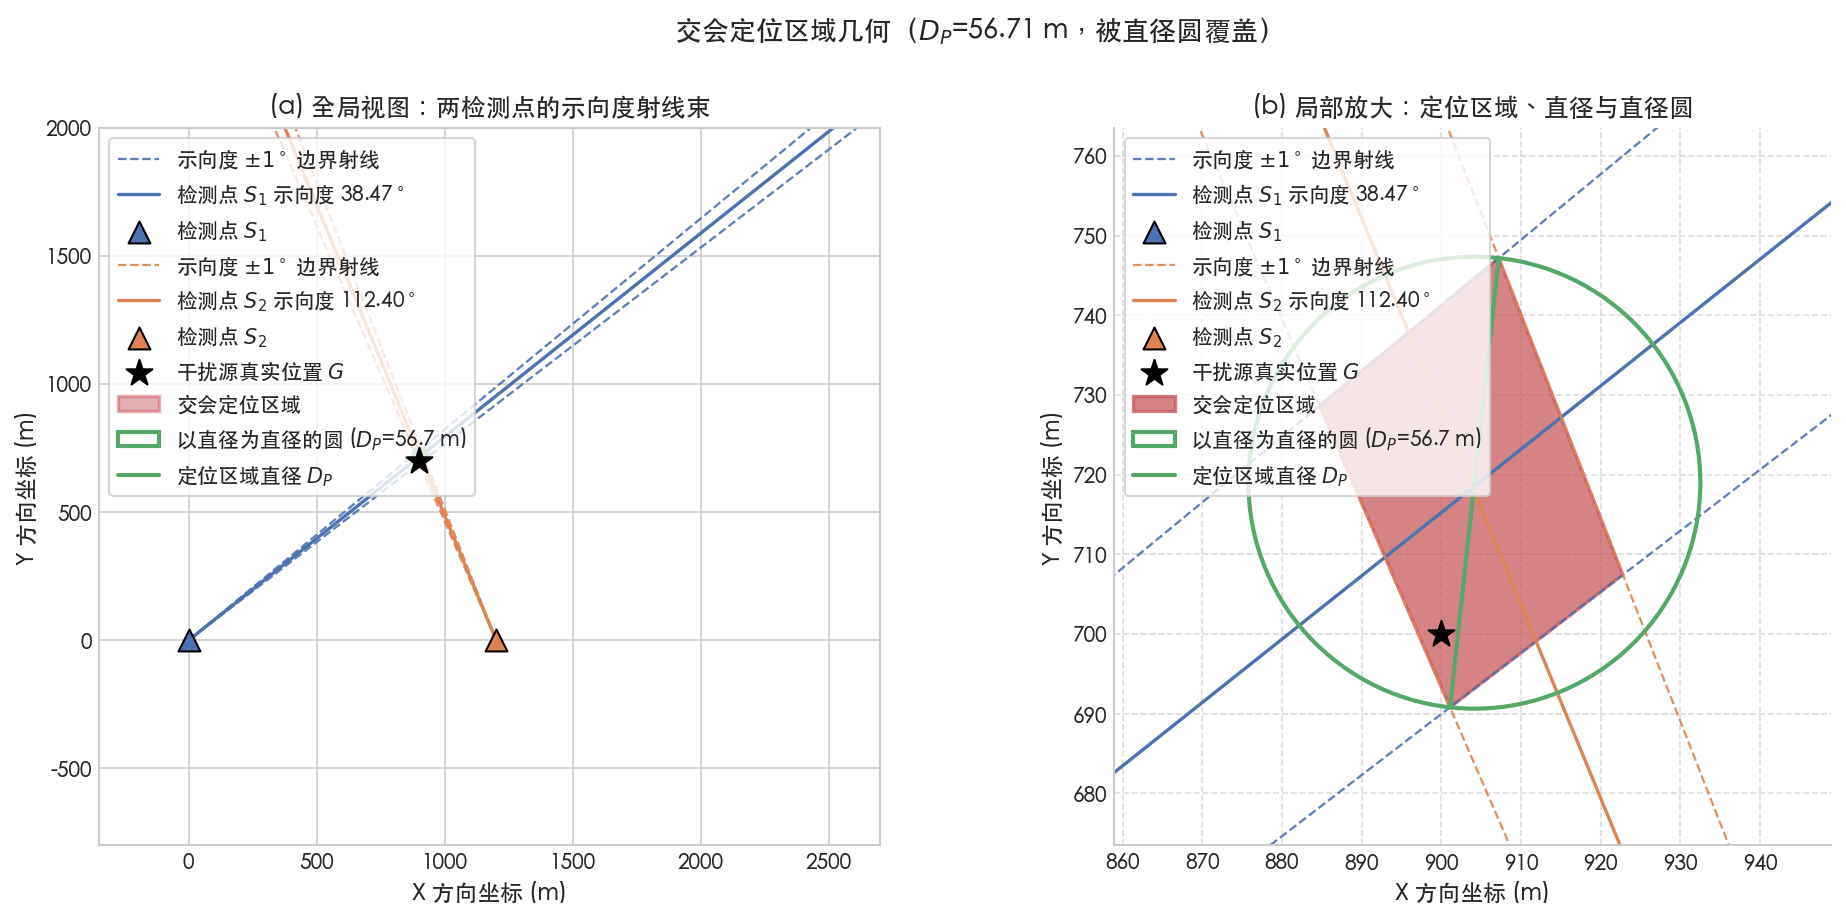
\includegraphics[width=0.8\textwidth]{问题一/figures/交会定位区域示意图.png}
  \caption{交会定位区域、直径与直径圆（示范构型）}
  \label{fig:p1-region}
\end{figure}

如图 \ref{fig:p1-region}(a) 所示，两条示向度射线束在目标附近相夹形成狭长的交集，该交集即定位区域；由于两条视线的交角较大，定位区域沿视线方向的延展被显著压缩。图 \ref{fig:p1-region}(b) 的局部放大显示，定位区域近似为一个平行四边形，其长对角线的中点恰好是直径圆的圆心，四个顶点几乎全部落在圆上。

\subsubsection{蒙特卡洛统计}

为回答"直径圆能否覆盖定位区域"这一具有普遍性的问题，本文在目标区域内随机生成检测点与干扰源，以真实方位角叠加 $U[-1^\circ,1^\circ]$ 的固定偏差构造示向度，得到 $5000$ 组构型。由于示向度由真实位置反推，真值必然落在定位区域内，构型始终具有物理意义。统计采用两种口径：纯交会四边形（即题目图 2 所示的红色四边形原型）与叠加目标圆域截断后的定位区域。结果如表 \ref{tab:p1-mc} 所示。

\begin{table}[H]
  \centering
  \caption{两种口径下的蒙特卡洛统计（各 5000 组构型）}
  \label{tab:p1-mc}
  \begin{tabularx}{\textwidth}{LCC}
    \toprule
    统计量 & 纯交会四边形 & 加目标圆域截断 \\
    \midrule
    非空构型占比 & $100.00\%$ & $100.00\%$ \\
    无界退化构型占比 & $2.80\%$ & $2.80\%$ \\
    有效构型数 & $4860$ & $4860$ \\
    \textbf{直径圆覆盖率} & $\mathbf{98.99\%}$ & $96.28\%$ \\
    直径均值 (m) & $402.53$ & $271.04$ \\
    直径中位数 (m) & $157.96$ & $151.88$ \\
    包围圆半径与直径之比（均值） & $0.500001$ & $0.5002$ \\
    包围圆半径与直径之比（最大） & $0.500280$ & $0.5611$ \\
    \bottomrule
  \end{tabularx}
\end{table}

由表 \ref{tab:p1-mc} 可见，纯交会口径下直径圆覆盖率为 $98.99\%$，且有界构型无一为空集；未加截断时约有 $2.8\%$ 的构型因两条视线近乎平行而退化无界，这部分构型在计入目标区域约束后自动变为有界，因此实际求解中截断是必需的。截断口径下覆盖率下降至 $96.28\%$，原因是定位区域与圆域边界相交后成为含圆弧边的多边形，圆弧段必然外凸于任何以其弦为直径的圆。

\begin{figure}[H]
  \centering
  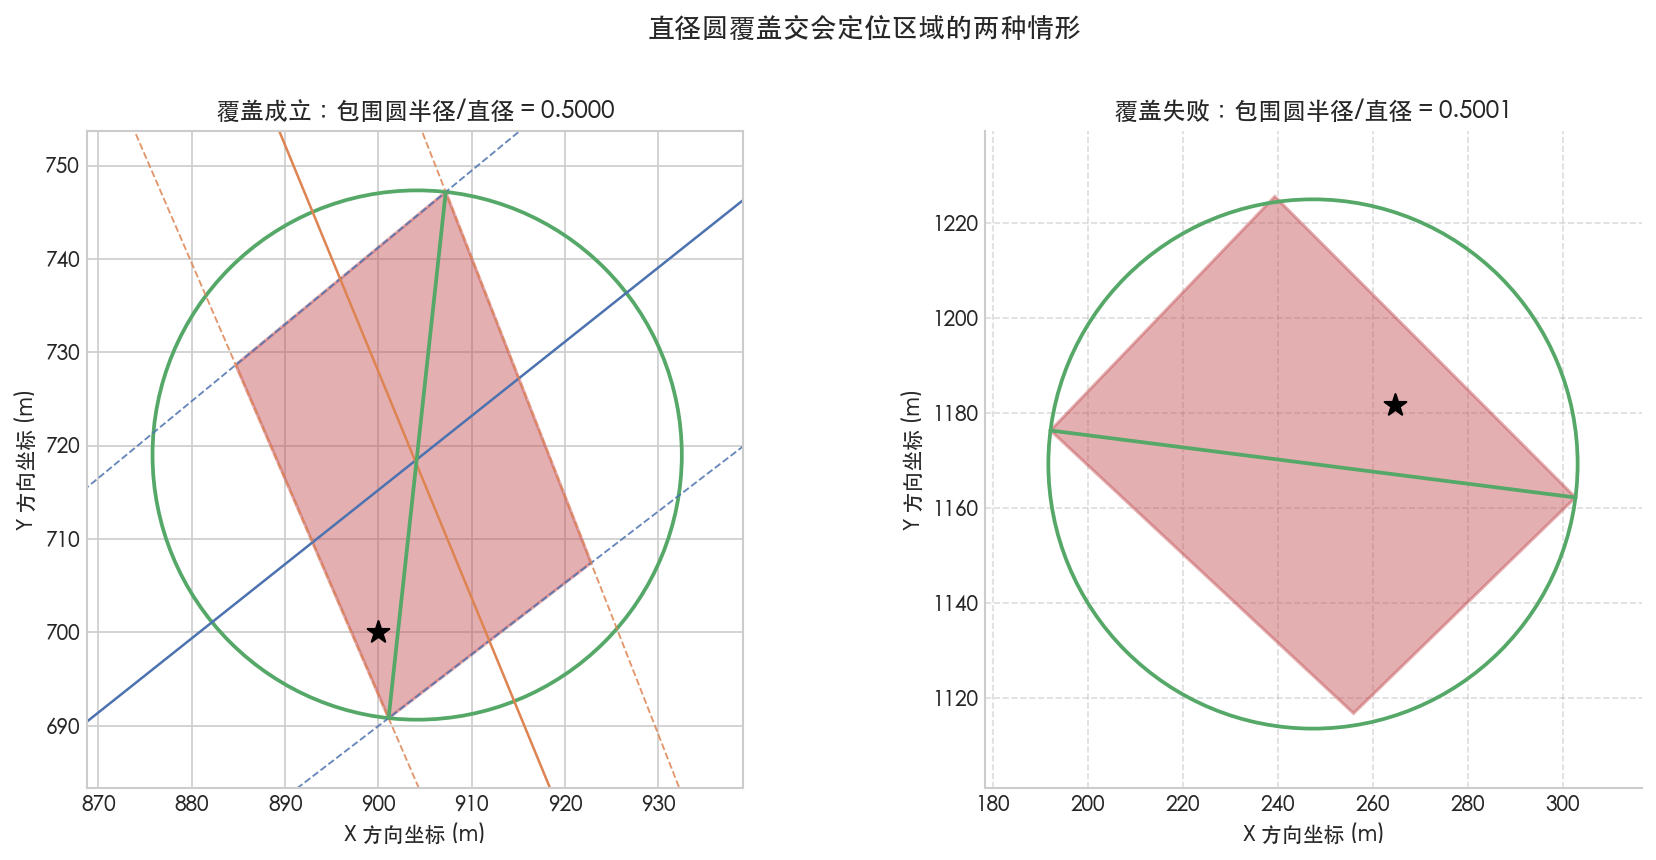
\includegraphics[width=0.8\textwidth]{问题一/figures/直径圆覆盖与不覆盖对比图.png}
  \caption{直径圆覆盖交会定位区域的两种情形}
  \label{fig:p1-cover}
\end{figure}

图 \ref{fig:p1-cover} 对比了覆盖成立与覆盖失败的两个真实算例。左图中定位区域近似为平行四边形，四个顶点全部落在直径圆内；右图取自蒙特卡洛中超出量最大的构型，该定位区域呈"菱形"状，其右侧顶点明显突出于直径圆之外，Thales 符号量一正一负，覆盖失败。

\subsubsection{覆盖率的结构与灵敏度}

将 $4860$ 个有效构型按两视线在干扰源处的交会角 $\alpha$ 分组统计，结果如表 \ref{tab:p1-group} 所示。

\begin{table}[H]
  \centering
  \caption{直径圆覆盖率按交会角分组统计（纯交会口径）}
  \label{tab:p1-group}
  \begin{tabular}{cccccc}
    \toprule
    交会角区间 & 构型数 & 直径均值 (m) & 直径中位数 (m) & 覆盖率 & 包围圆半径/直径均值 \\
    \midrule
    $(0^\circ,30^\circ]$   & $1486$ & $950.26$ & $499.79$ & $100.00\%$ & $0.5000$ \\
    $(30^\circ,45^\circ]$  & $688$  & $201.55$ & $200.85$ & $100.00\%$ & $0.5000$ \\
    $(45^\circ,60^\circ]$  & $568$  & $136.17$ & $134.21$ & $100.00\%$ & $0.5000$ \\
    $(60^\circ,75^\circ]$  & $482$  & $106.85$ & $107.16$ & $100.00\%$ & $0.5000$ \\
    $(75^\circ,90^\circ]$  & $404$  & $83.50$  & $85.25$  & $98.02\%$  & $0.5000$ \\
    $(90^\circ,105^\circ]$ & $342$  & $76.21$  & $77.74$  & $88.01\%$  & $0.5000$ \\
    $(105^\circ,120^\circ]$& $231$  & $84.82$  & $87.31$  & $100.00\%$ & $0.5000$ \\
    $(120^\circ,150^\circ]$& $363$  & $111.35$ & $112.21$ & $100.00\%$ & $0.5000$ \\
    $(150^\circ,180^\circ]$& $296$  & $530.07$ & $299.21$ & $100.00\%$ & $0.5000$ \\
    \bottomrule
  \end{tabular}
\end{table}

表 \ref{tab:p1-group} 揭示了一个清晰的结构：覆盖率仅在交会角接近 $90^\circ$ 的区间出现明显下降，其余区间均为 $100\%$。其几何原因在于，当两视线正交时，两个张角为 $2^\circ$ 的锥相交所得的四边形趋近于矩形，而矩形正是 Thales 判据的临界形状——四个内角恰为 $90^\circ$、四个顶点恰好落在直径圆上；真实锥形带来的微小扰动使其中某个顶点稍微外移或内移，于是覆盖与否各占一定比例。当交会角显著偏离 $90^\circ$ 时，定位区域变为"长菱形"，由前述等价条件可知长对角线的两个端点处内角一个变钝一个变锐，整体仍满足覆盖判据。图中还显示，交会角越小则定位区域直径越大，$(0^\circ,30^\circ]$ 区间的直径均值接近 $1$ 千米，这正是交会几何变差的直接体现。

\begin{figure}[H]
  \centering
  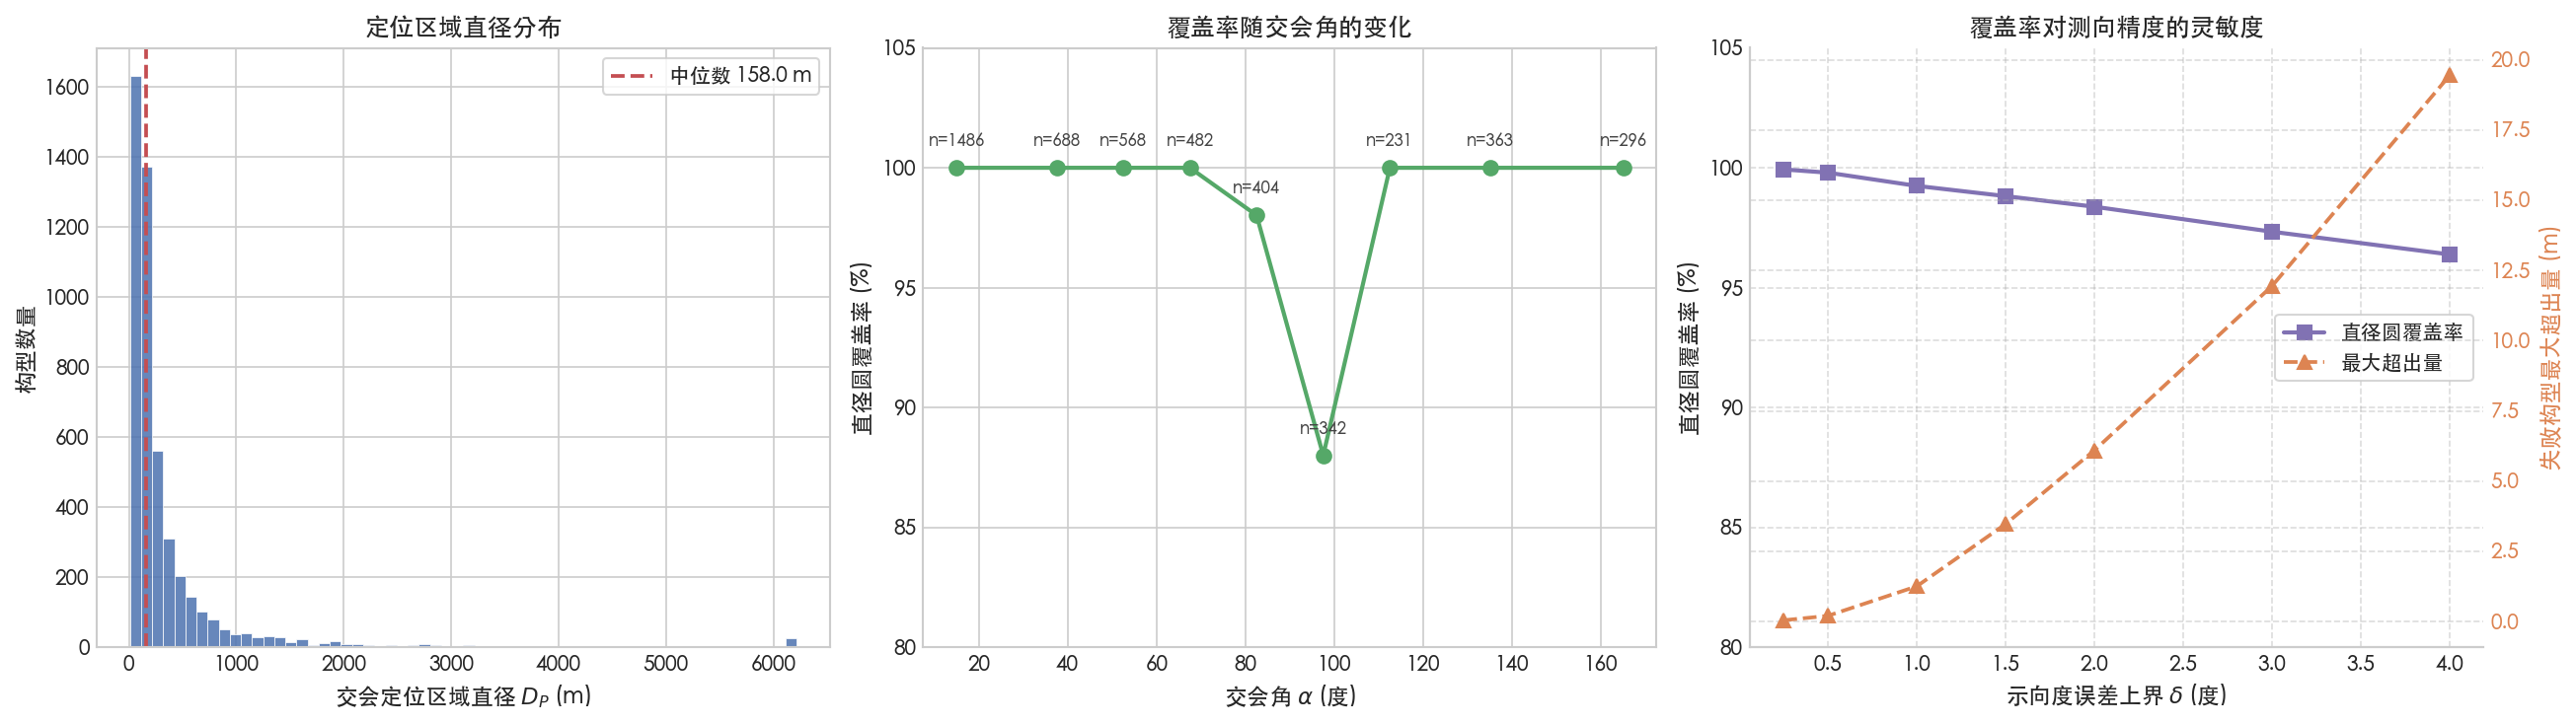
\includegraphics[width=0.8\textwidth]{问题一/figures/直径圆覆盖率与直径分布图.png}
  \caption{定位区域直径分布、覆盖率随交会角的变化与测向精度灵敏度}
  \label{fig:p1-stat}
\end{figure}

图 \ref{fig:p1-stat}(a) 显示定位区域直径呈显著右偏分布，中位数约 $158$ 米而均值超过 $400$ 米，说明大部分构型下定位精度尚可，但存在少量直径达千米量级的劣质构型。图 \ref{fig:p1-stat}(b) 直观呈现了覆盖率在 $90^\circ$ 附近的凹陷。图 \ref{fig:p1-stat}(c) 给出覆盖率对测向精度上界 $\delta$ 的灵敏度：当 $\delta$ 由 $1^\circ$ 收紧至 $0.25^\circ$ 时覆盖率升至 $99.93\%$，放宽至 $4^\circ$ 时降至 $96.39\%$，同时失败构型的最大超出量由 $1.17$ 米增至 $19.45$ 米。需要强调的是，全部失败构型中顶点超出直径圆的最大距离仅为 $1.1697$ 米，平均仅 $0.4928$ 米，占定位区域直径的比例不超过 $1.37\%$。

综上，问题一的结论是：以定位区域直径为直径的圆\textbf{不能保证}覆盖定位区域，其成立的充要条件是式 \eqref{eq:thales-condition}；在满足有界性的随机交会构型中，覆盖成立的频率约为 $98.99\%$，失效仅发生在交会角接近 $90^\circ$ 的临界构型上，且失效的绝对幅度不超过米级，对后续以 $20$ 米清除半径为精度要求的任务而言影响可以忽略。

% ==================================================================
\section{问题二：第二个检测点的选择策略与候选区域}
% ==================================================================

\subsection{具体分析}

问题二要求在某全向干扰源已被一个检测点测得示向度的条件下，给出第二个检测点的选择策略与候选区域。该问题属于带不确定性的实验设计类问题：决策变量是第二个检测点的平面位置，目标函数是该点的观测所带来的定位精度增益。其难点根源于单站方位观测的信息贫乏性——一条示向度只把干扰源约束在张角 $2^\circ$ 的楔形内，沿视线方向的径向不确定度可达上千米；同时目标距离完全未知，使得经典的"已知目标位置时的最优交会布站"结论无法直接套用，必须在可行域上改用期望或极小化极大准则重新求解，并把单点最优松弛为一片候选区域以便工程实施。

\subsection{模型准备}

\subsubsection{可行域的建立与坐标归一化}

作刚性变换：把第一个检测点 $S_1$ 平移至坐标原点，并把示向度方向旋转至 $+x$ 轴。变换后干扰源 $G$ 的可行域为
\begin{equation}
\Omega=\Bigl\{\,G=r\,u(a):\ 0<r\le r_{\mathrm{hi}},\ \lvert a\rvert\le\delta\,\Bigr\},
\qquad r_{\mathrm{hi}}=\min\left\{R_{c}^{\max},\ r_{\partial}\right\},
\label{eq:omega}
\end{equation}
其中 $r_{\mathrm{hi}}$ 为径向可行上界，$R_c^{\max}=1500$ 米为有效接收半径的上界，$r_{\partial}$ 为沿该方向到目标区域边界的距离；由于被测到信号意味着干扰源必然在有效接收半径之内，故 $r\le1500$ 米是硬约束。

\subsubsection{算法选择}

候选区域与最优基线可以由三种途径得到。解析法通过误差传播公式求极值，可给出闭式结论但只能处理简单布站形式；数值优化法在二维决策空间上直接搜索，通用但可能陷入局部最优；贝叶斯方法把距离作为待估参数求后验方差，理论最优但需要完整的先验分布且计算量大。本文采用"解析求特例 $+$ 数值求一般"的组合策略：先用解析法给出垂直布站这一特殊形式下的完整闭式解，作为理解问题结构与验证数值结果的标尺；再在 $(b,\varphi)$ 二维空间上做网格粗搜加 Nelder--Mead 精搜，处理一般形式的布站决策；最后以次水平集的形式给出候选区域。两者的适用性对比见表 \ref{tab:p2-algo}。

\begin{table}[H]
  \centering
  \caption{第二检测点布站决策方法的对比}
  \label{tab:p2-algo}
  \begin{tabularx}{\textwidth}{CCL}
    \toprule
    方法 & 优点 & 限制 \\
    \midrule
    误差传播解析极值 & 结论闭式、可解释性强 & 只适用于垂直布站等简单形式 \\
    二维网格 $+$ 局部精搜 & 通用、可给出全域结构 & 依赖网格分辨率，需验证全局性 \\
    后验方差最小化 & 理论上最优 & 需给定距离先验，计算成本高 \\
    \bottomrule
  \end{tabularx}
\end{table}

\subsection{模型建立}

\subsubsection{误差传播公式}

设第二检测点 $S_2=S_1+b\,u(\varphi)$，即基线长度为 $b$、基线方向与示向度方向夹角为 $\varphi$。记干扰源到两检测点的距离为 $r_1=\lvert S_1G\rvert$、$r_2=\lvert S_2G\rvert$，$G$ 处两视线的交会角为 $\alpha$。当两条方位线分别因环境偏差而产生角扰动 $\delta\varphi_1,\delta\varphi_2$ 时，把方位线视为绕站点旋转，则第 $i$ 条线旋转 $\delta\varphi_i$ 会使交点沿另一条线的方向移动 $r_i\delta\varphi_i/\sin\alpha$，于是交点位移为
\begin{equation}
\Delta P=\frac{r_1\,\delta\varphi_1}{\sin\alpha}\,\hat u_2+\frac{r_2\,\delta\varphi_2}{\sin\alpha}\,\hat u_1,
\label{eq:err-vec}
\end{equation}
式中 $\hat u_i$ 为第 $i$ 条方位线的单位方向向量。取最坏组合 $\lvert\delta\varphi_1\rvert=\lvert\delta\varphi_2\rvert=\delta$ 且同号，得定位偏差上界
\begin{equation}
E(S_2;G)=\frac{\delta}{\sin\alpha}\sqrt{r_1^2+r_2^2+2r_1r_2\cos\alpha}.
\label{eq:err-general}
\end{equation}
式 \eqref{eq:err-general} 把布站决策完全归结为交会角与两站距离的组合，是后续全部优化的基础。需要特别指出，当三点共线时 $\sin\alpha\to0$，$E\to\infty$，其物理含义是共线观测无法提供任何距离信息，这正是"沿视线方向径直逼近"策略失效的根本原因。

\subsubsection{垂直布站的解析最优}

对垂直布站这一自然选择，即取 $\varphi=90^\circ$，由余弦定理可得 $\cos\alpha=r_1/r_2$ 且 $\sin\alpha=b/r_2$，代入式 \eqref{eq:err-general} 化简为
\begin{equation}
E(b;r)=\frac{\delta}{b}\sqrt{(r^2+b^2)(4r^2+b^2)} .
\label{eq:err-perp}
\end{equation}
令 $t=b^2/r^2$，则 $E\propto\sqrt{t+5+4/t}$，该函数在 $t=2$ 处取得唯一极小值 $3$。由此得到本问的核心解析结论
\begin{equation}
\boxed{\quad b^{*}=\sqrt2\,r,\qquad
\alpha^{*}=\arccos\frac{1}{\sqrt3}=54.74^\circ,\qquad
E_{\min}=3\delta r\approx0.052360\,r \quad}
\label{eq:opt-b}
\end{equation}
该结论的物理含义值得强调：最优交会角并非教科书中常被引用的 $90^\circ$，而是 $54.74^\circ$。其原因是误差传播式 \eqref{eq:err-general} 中两条方位线的贡献分别被 $r_1$ 与 $r_2$ 加权，在 $b=\sqrt2r$ 处二者的加权和达到均衡；若强行取 $90^\circ$ 交会，则代价是基线必须放长，$r_2$ 增大反而放大了第二条方位线的误差贡献。

\subsubsection{稳健准则与候选区域}

由于实际情形中 $r$ 未知，式 \eqref{eq:opt-b} 只能视作以估计值 $\hat r$ 代入的近似最优，必须引入稳健化准则。

极小化极大准则注意到式 \eqref{eq:err-perp} 关于 $r$ 单调递增，故最坏情形取在 $r_{\mathrm{hi}}$ 处：
\begin{equation}
b_{\mathrm{mm}}=\arg\min_{b}\max_{r\in[r_{\mathrm{lo}},r_{\mathrm{hi}}]}E(b;r)=\sqrt2\,r_{\mathrm{hi}} .
\label{eq:minimax}
\end{equation}

期望准则设 $r$ 在可行域内按面积均匀分布，即密度函数 $f(r)=2r/r_{\mathrm{hi}}^2$，则
\begin{equation}
b_{\mathrm{exp}}=\arg\min_{b}\int_{r_{\mathrm{lo}}}^{r_{\mathrm{hi}}}\frac{\delta}{b}\sqrt{(r^2+b^2)(4r^2+b^2)}\;\frac{2r}{r_{\mathrm{hi}}^2}\,\mathrm{d}r .
\label{eq:expect}
\end{equation}
更一般地，把 $\varphi$ 一并放开，在可行域上取期望定位误差作为目标函数：
\begin{equation}
J(S_2)=\mathbb E_{G\sim U(\Omega)}\bigl[\,E(S_2;G)\,\bigr]
=\frac{1}{\lvert\Omega\rvert}\int_{\Omega}E(S_2;G)\,\mathrm{d}G .
\label{eq:objective}
\end{equation}

候选区域定义为目标函数 \eqref{eq:objective} 关于最优值的次水平集：
\begin{equation}
\mathcal C=\Bigl\{\,S_2:\ J(S_2)\le(1+\varepsilon)J(S_2^{*})\,\Bigr\},
\qquad \varepsilon=5\%,
\label{eq:candidate-region}
\end{equation}
即允许定位误差相对最优值最多退化 $5\%$ 的全部布站位置构成的区域。这一表述的工程价值在于，它把"唯一最优点"松弛为"一片可接受区域"，使机器狗能够结合地形、障碍与其他任务需求在区域内灵活选取实际站位。

\subsection{模型求解}

\subsubsection{解析结论的数值核对}

表 \ref{tab:p2-ana} 给出垂直布站解析最优的数值核对结果。对 $r$ 从 $200$ 米到 $1500$ 米逐点做一维精细搜索，最优基线与 $r$ 的比值稳定在 $1.414213\sim1.414226$，与解析值 $\sqrt2$ 的相对偏差小于 $10^{-5}$；最优交会角稳定在 $54.73^\circ\sim54.74^\circ$；最小误差与 $r$ 的比值恒为 $0.052360$，与解析系数 $3\delta$ 完全吻合。解析结论得到严格验证。

\begin{table}[H]
  \centering
  \caption{垂直布站解析最优的数值核对}
  \label{tab:p2-ana}
  \begin{tabular}{cccccc}
    \toprule
    源距离 $r$ (m) & 最优基线 $b^*$ (m) & $b^*/r$ & 最优交会角 & 最小误差 $E_{\min}$ (m) & $E_{\min}/r$ \\
    \midrule
    $200$  & $282.84$  & $1.414201$ & $54.735^\circ$ & $10.472$  & $0.052360$ \\
    $600$  & $848.53$  & $1.414217$ & $54.736^\circ$ & $31.416$  & $0.052360$ \\
    $1000$ & $1414.21$ & $1.414210$ & $54.736^\circ$ & $52.360$  & $0.052360$ \\
    $1400$ & $1979.90$ & $1.414214$ & $54.736^\circ$ & $73.304$  & $0.052360$ \\
    $1500$ & $2121.33$ & $1.414217$ & $54.736^\circ$ & $78.540$  & $0.052360$ \\
    \bottomrule
  \end{tabular}
\end{table}

\begin{figure}[H]
  \centering
  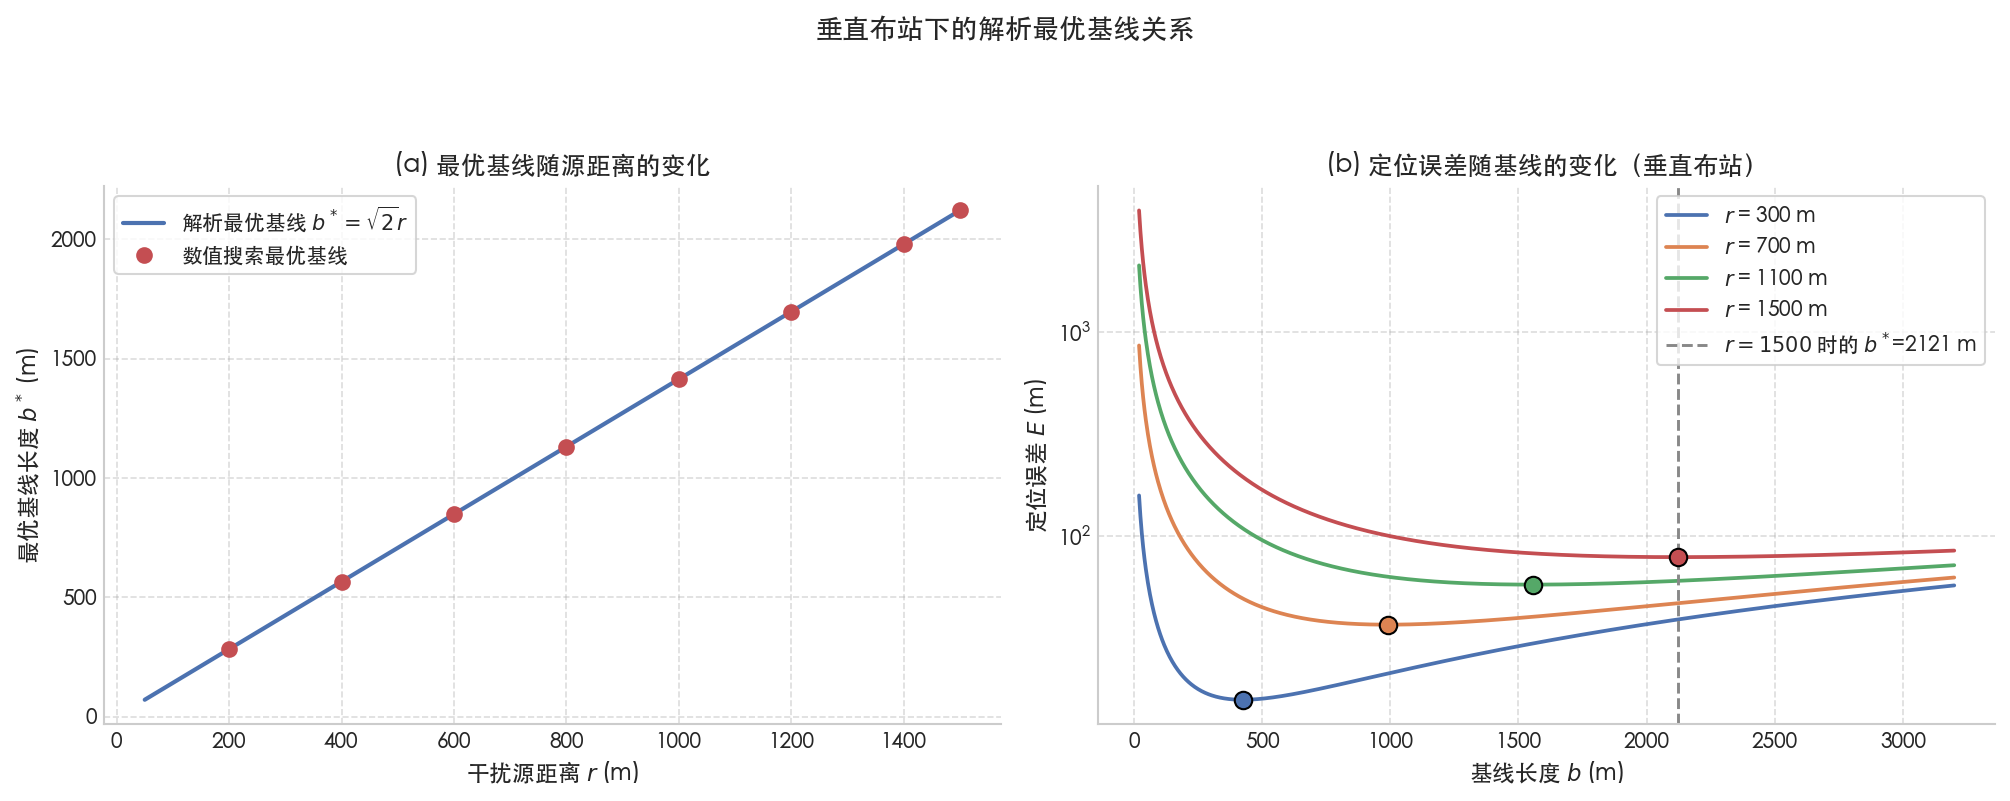
\includegraphics[width=0.8\textwidth]{问题二/figures/最优基线与距离关系图.png}
  \caption{垂直布站下最优基线与源距离的解析关系及误差曲线}
  \label{fig:p2-ana}
\end{figure}

图 \ref{fig:p2-ana}(a) 显示数值搜索得到的最优基线与解析直线 $b^*=\sqrt2r$ 完全重合；图 \ref{fig:p2-ana}(b) 给出不同源距离下误差随基线的变化曲线，每条曲线均呈"先降后升"的 U 形，极小点位置随 $r$ 线性外移，且最小值随 $r$ 线性增大，直观印证了式 \eqref{eq:opt-b}。

\subsubsection{一般布站的数值最优}

在可行域 $\Omega$ 内按面积均匀采样 $8000$ 个候选源位置，对每个候选布站位置计算期望定位误差 \eqref{eq:objective}，在 $(b,\varphi)$ 极坐标网格（$b$ 步长 $25$ 米、$\varphi$ 步长 $1.5^\circ$）上粗搜后再用 Nelder--Mead 单纯形法精搜。所得最优布站如表 \ref{tab:p2-opt} 所示。

\begin{table}[H]
  \centering
  \caption{三种准则下的最优布站与定位精度}
  \label{tab:p2-opt}
  \begin{tabularx}{\textwidth}{LCCCC}
    \toprule
    准则 & 最优基线 $b^*$ (m) & 最优方位角 $\varphi^*$ & 期望误差 (m) & 最坏误差 (m) \\
    \midrule
    期望准则（主） & $1401.4$ & $20.03^\circ$ & $\mathbf{22.19}$ & $72.87$ \\
    极小化极大准则 & $1499.3$ & $41.09^\circ$ & $26.90$ & $\mathbf{39.92}$ \\
    限定垂直布站（次优） & $1510.0$ & $90.00^\circ$ & $55.73$ & $83.80$ \\
    \bottomrule
  \end{tabularx}
\end{table}

表 \ref{tab:p2-opt} 给出了一个在直觉上颇具冲击力的结果：在计入全可行域不确定性后，最优布站并非垂直，而是取 $\varphi^*\approx20^\circ$、$b^*\approx1401$ 米，此时期望定位误差为 $22.19$ 米；而教科书式的垂直布站即使把基线放长到 $1510$ 米，期望误差仍高达 $55.73$ 米，是最优方案的 $2.5$ 倍。若采用极小化极大准则，则最优位置向垂直方向移动至 $\varphi^*=41.09^\circ$、$b^*=1499.3$ 米，期望误差略有上升但最坏误差由 $72.87$ 米压缩至 $39.92$ 米，体现出"平均最优"与"最坏最优"之间的典型权衡。

\begin{figure}[H]
  \centering
  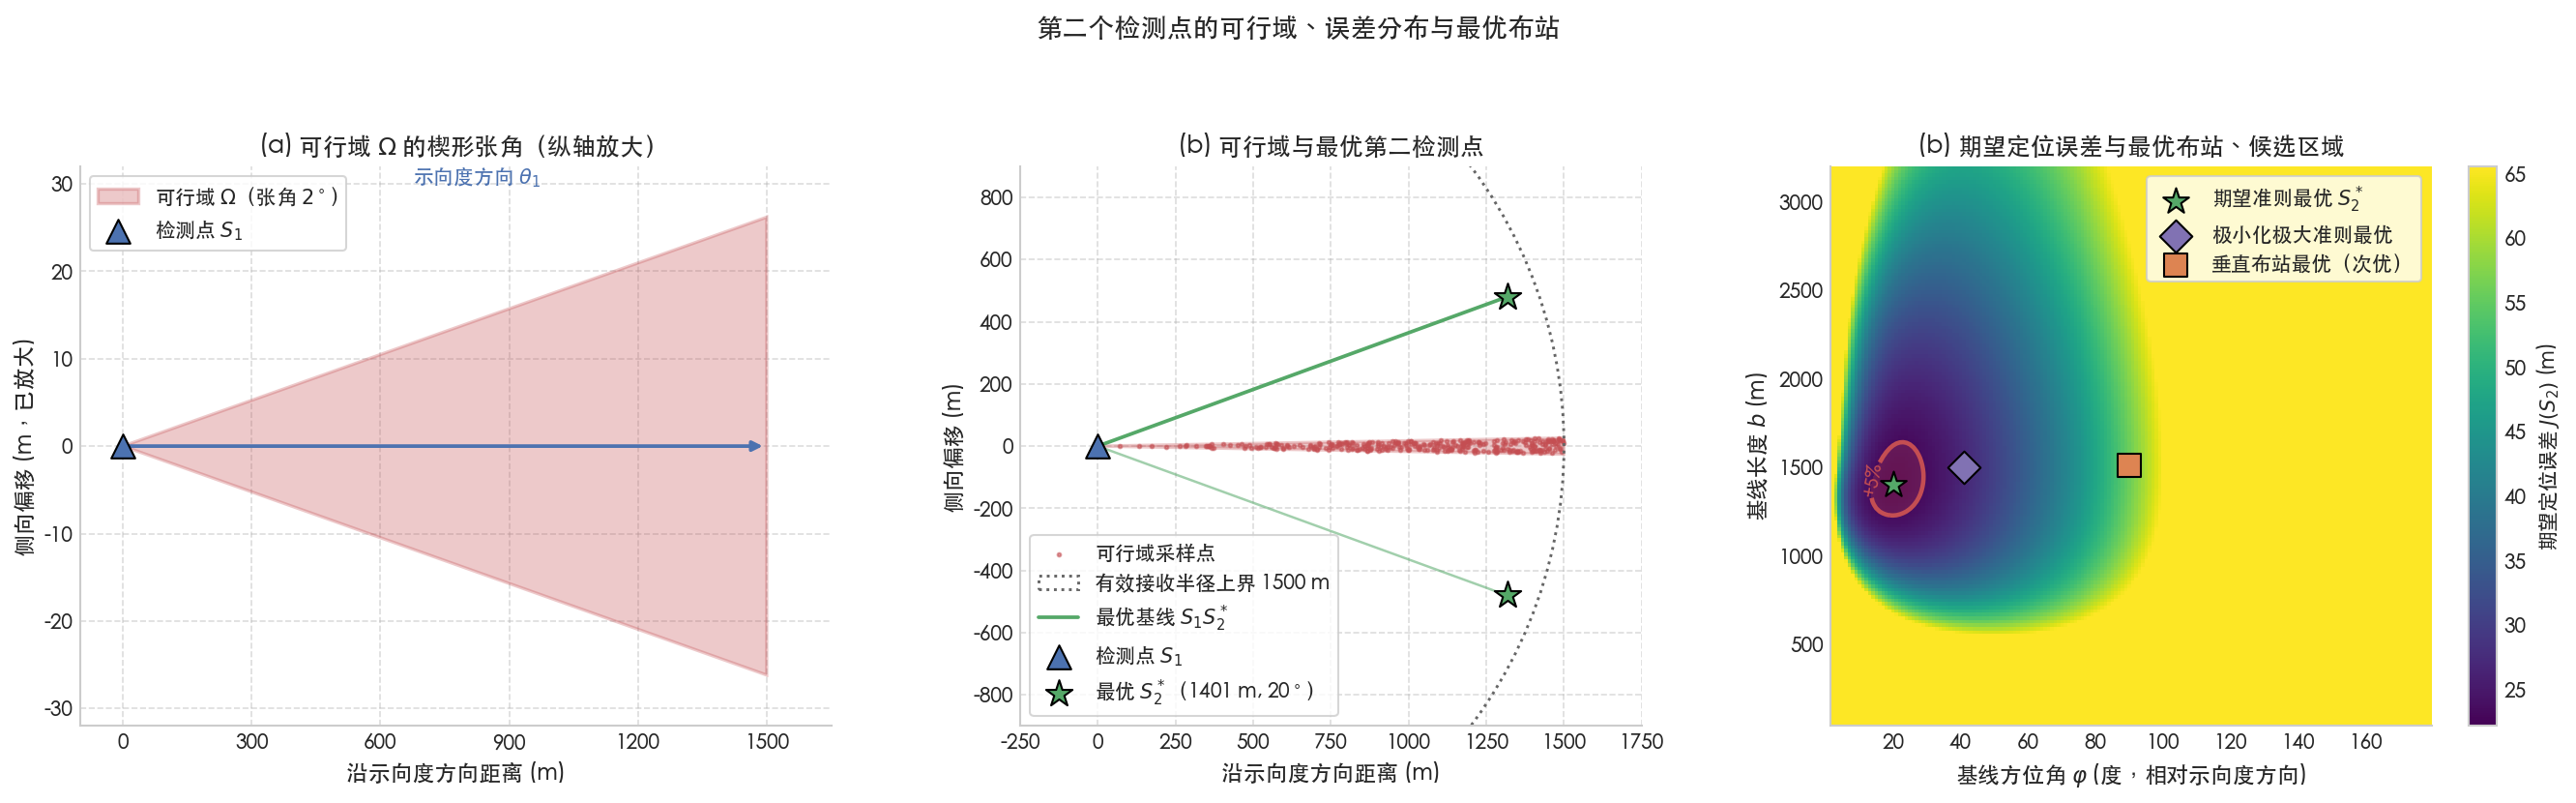
\includegraphics[width=0.8\textwidth]{问题二/figures/可行域与候选区域示意图.png}
  \caption{干扰源可行域、定位误差分布与最优第二检测点}
  \label{fig:p2-field}
\end{figure}

图 \ref{fig:p2-field}(a) 以放大纵轴的方式呈现了可行域的张角结构：张角仅 $2^\circ$，在 $1500$ 米处侧向宽度仅约 $52$ 米，这种极度扁平的形状正是径向不确定度巨大而侧向信息几乎确定的几何体现。图 \ref{fig:p2-field}(b) 把可行域与最优第二检测点叠置显示，最优位置位于视线方向前出约 $1401$ 米、侧偏约 $479$ 米处。图 \ref{fig:p2-field}(c) 是 $(b,\varphi)$ 平面上的期望误差热力图：误差最小值出现在 $\varphi\approx20^\circ$、$b\approx1400$ 米附近，图中同时标出三种准则的最优解，并以阴影标出候选区域。

\begin{figure}[H]
  \centering
  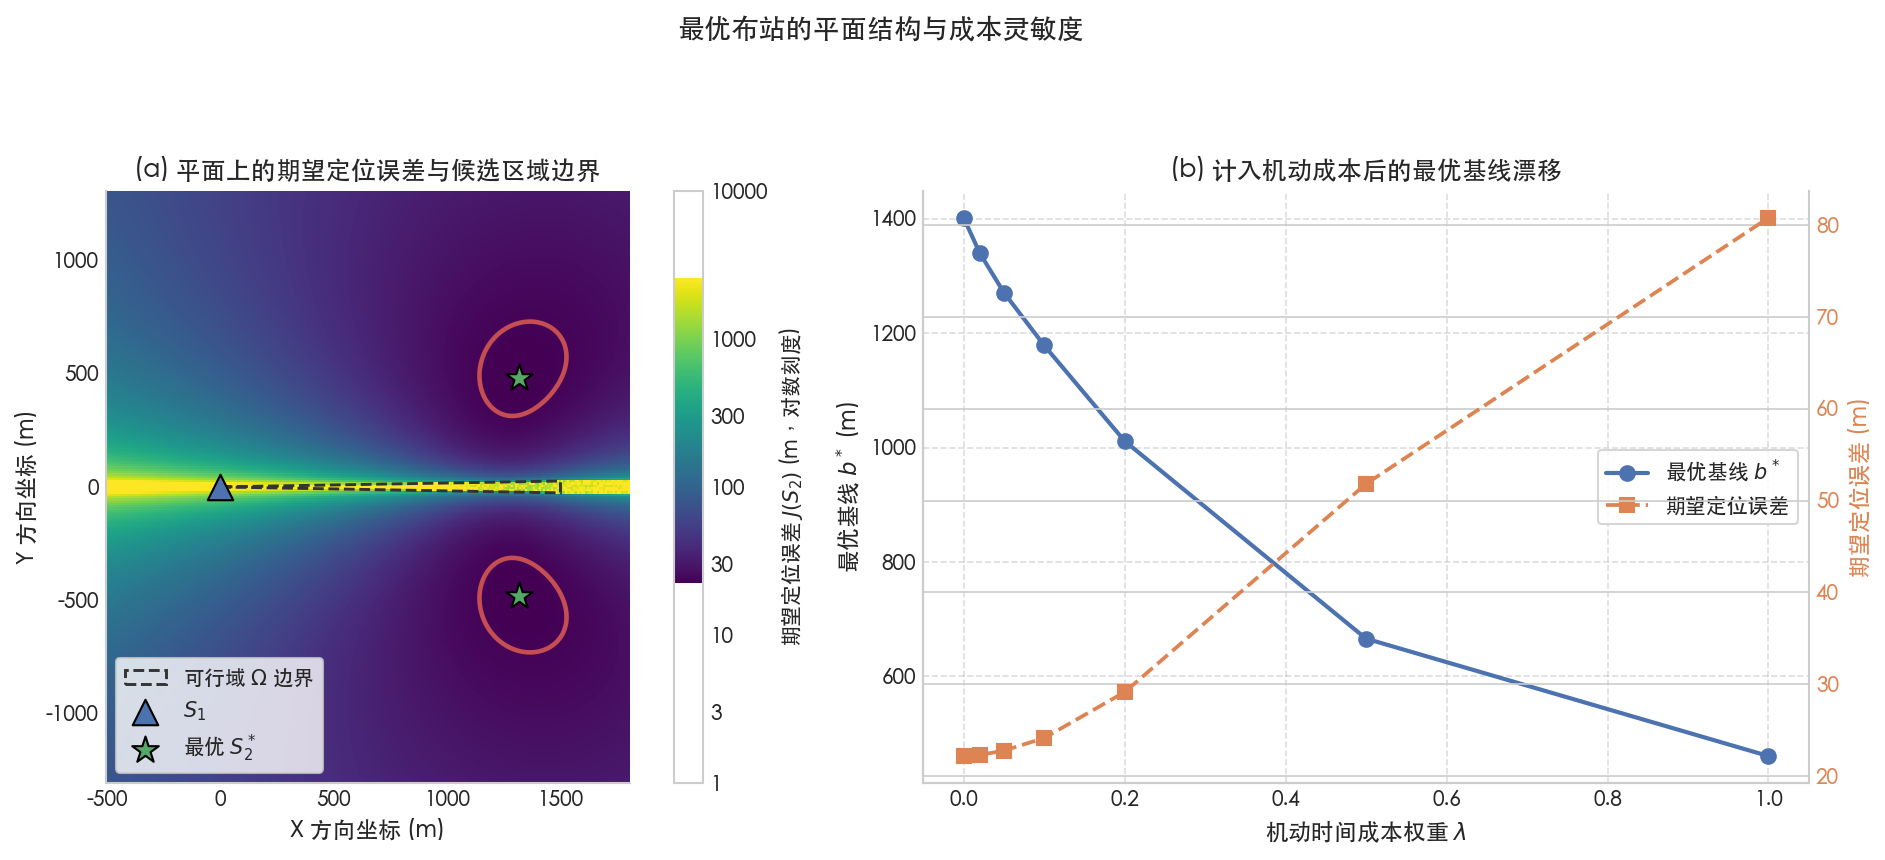
\includegraphics[width=0.8\textwidth]{问题二/figures/最优布站平面结构与成本灵敏度图.png}
  \caption{平面上的期望定位误差结构与机动成本灵敏度}
  \label{fig:p2-plane}
\end{figure}

图 \ref{fig:p2-plane}(a) 把目标函数铺展到整个平面上，色标取对数刻度。图中沿示向度方向存在一条明亮的高误差脊线，其成因正是共线观测导致的 $\sin\alpha\to0$；脊线两侧对称地分布着两个低误差"盆地"，最优第二检测点落于其中。这一结构清楚地说明，第二检测点必须"避开视线、侧向展开"，而侧向展开到什么程度则由径向不确定性与探测几何共同决定。

\subsubsection{候选区域}

取 $\varepsilon=5\%$ 的容差，由式 \eqref{eq:candidate-region} 求解得到候选区域为
\begin{equation}
\mathcal C:\quad b\in[1230,\ 1630]\ \text{m},\qquad
\varphi\in[14^\circ,\ 29^\circ]\ \ (\text{含关于视线方向的镜像}).
\label{eq:cand-result}
\end{equation}
即第二个检测点应选在以第一检测点为圆心、半径 $1230\sim1630$ 米、偏离示向度方向 $14^\circ\sim29^\circ$ 的两条对称圆弧带内，其对称轴方向为 $\theta_1\pm\varphi^*$。该区域以约 $400$ 米的径向宽度换取了不超过 $5\%$ 的定位精度损失，为实际布站留出了充分的工程余量。

\subsubsection{机动成本灵敏度}

问题二本身未计入机器狗的机动代价，但由问题三可知移动时间往往是虚拟时间的主要成分，故有必要考察"计入单位机动成本 $\lambda\lvert S_2\rvert/v$"后最优基线的漂移。取 $\lambda$ 从 $0$ 递增至 $1.0$，结果如表 \ref{tab:p2-lam} 所示。

\begin{table}[H]
  \centering
  \caption{计入机动时间成本后的最优布站漂移}
  \label{tab:p2-lam}
  \begin{tabular}{cccccc}
    \toprule
    成本权重 $\lambda$ & $0$ & $0.05$ & $0.1$ & $0.5$ & $1.0$ \\
    \midrule
    最优基线 $b^*$ (m) & $1401$ & $1271$ & $1179$ & $666$ & $461$ \\
    最优方位角 $\varphi^*$ & $20.0^\circ$ & $19.5^\circ$ & $20.5^\circ$ & $43.1^\circ$ & $56.3^\circ$ \\
    期望定位误差 (m) & $22.19$ & $22.78$ & $24.15$ & $51.83$ & $80.79$ \\
    \bottomrule
  \end{tabular}
\end{table}

表 \ref{tab:p2-lam} 显示，当机动成本较小时（$\lambda\le0.1$）最优基线基本不变，说明定位精度对基线长度在最优值附近并不敏感；但当成本权重进一步增大时，基线迅速收缩且方位角向 $54.74^\circ$ 靠拢——这恰好是式 \eqref{eq:opt-b} 给出的解析最优交会角，说明"短基线"必须搭配"接近最优交会角"的方位才能维持可接受的精度。该结论为问题三中采用"短侧移 $+$ 逐步逼近"的折中策略提供了理论依据。

% ==================================================================
\section{问题三：全向干扰源的搜索、定位与清除策略}
% ==================================================================

\subsection{具体分析}

问题三要求在干扰源个数未知（$10\sim16$ 个）、位置未知、频道未知的条件下，为机器狗制定从原点出发、初始频道为 $1$ 的自动搜索定位与清除策略，在确保全部清除的前提下最小化任务时间。该问题属于不完全观测条件下的序贯决策问题：观测算子只返回角度且叠加 $1^\circ$ 误差，目标个数与位置先验完全未知，决策变量是"下一步去哪里、测哪个频道"。

问题的结构可以分解为三个层次。第一层是探测的可达性，任何干扰源只有落在某个观测点的有效接收半径内且在其覆盖角内才能被察觉，而有效接收半径在 $1000\sim1500$ 米之间且具体数值未知，因此必须设计对半径取最坏情形仍成立的观测点集。第二层是定位的欠定性，单次示向度只给出方向，必须至少两次不同位置的观测才能解算位置，而两次观测的几何关系直接决定定位精度。第三层是清除的距离约束，激光清除要求机器狗与干扰源的距离不超过 $20$ 米，因此定位精度必须优于该阈值。三个层次通过虚拟时间串联：探测次数消耗固定检测时间，定位机动消耗移动时间，逼近与清除消耗另一部分时间，策略设计本质上是在这三项之间做最优分配。

关于时间口径需要先行澄清。题目中"定位清除总时间包含机器狗移动时间、频道切换时间、检测时间、光学精确定位时间及清除时间"，这些量均由模拟器按虚拟世界时钟累计；而 $20$ 分钟的程序运行时间限制针对的是机器狗程序在现实世界中的运行时长。因此在虚拟时间上限 $360000$ 秒（$100$ 小时）之内，真正需要最小化的量是虚拟时间之和，现实时间限制仅要求程序本身足够高效。

\subsection{模型准备}

\subsubsection{可检测性模型与预处理的参数整理}

由附录 2，全向干扰源 $G_c$（频道 $c$）在检测点 $P$ 处可被检测的充要条件为 $\lVert P-G_c\rVert\le r_c$，其中有效接收半径 $r_c\in[1000,1500]$ 且不通过接口返回。由于 $r_c$ 的具体取值未知，本文采用最坏情形口径：若观测点集 $\mathcal Q$ 满足
\begin{equation}
\forall X\in D,\quad \exists Q\in\mathcal Q:\ \lVert X-Q\rVert\le R_c^{\min}=1000,
\label{eq:cover-cond}
\end{equation}
则无论各干扰源的真实 $r_c$ 取何值，目标区域内的任何干扰源都至少能被 $\mathcal Q$ 中某一点测到。式 \eqref{eq:cover-cond} 把"保证可测"问题化归为一个纯粹的圆覆盖问题：用半径 $1000$ 米的圆盘覆盖半径 $1800$ 米的圆域 $D$。

在进入求解前，先将全部常量、坐标与时间参数统一整理为程序可读的形式，并把示向度与坐标的约定统一为"正东为 $x$ 轴正向、逆时针为正"，以避免接口参数与内部计算之间的符号错误；同时对全部可能超界的坐标分量做 $2\times10^6$ 米的范围校核。这一步虽无复杂的数学内容，却是程序正确性的前提。

\subsubsection{算法选择}

搜索策略的设计有三条技术路线。全覆盖扫描法把目标区域离散为满足保证可测条件的观测点集，逐点扫描全部频道，优点是"确保全部清除"这一硬约束天然成立，缺点是需要为覆盖率付出行程代价。概率搜索法借助先验分布做贝叶斯序贯探测，在目标分布已知时可显著提高效率，但本题对干扰源分布没有任何先验信息，无法建立有效的后验更新。主动探测与信息增益法以最大化信息熵减少量为准则选择下一个观测点，理论上最优但需要维护一个高维信念状态，在 $100$ 米量级的定位精度要求下计算量不可接受。综合考虑硬约束的满足性与计算的可行性，本文选择"保证覆盖网 $+$ 分层闭环"的技术路线，并以旅行商下界作为策略优劣的评判标尺。

\begin{table}[H]
  \centering
  \caption{搜索策略技术路线的对比}
  \label{tab:p3-algo}
  \begin{tabularx}{\textwidth}{CCL}
    \toprule
    路线 & 优点 & 限制 \\
    \midrule
    保证覆盖网扫描 & 满足"确保全部清除"的硬约束 & 需求解覆盖网并付出扫描行程 \\
    贝叶斯序贯探测 & 有先验时效率高 & 本题无目标分布先验 \\
    信息增益主动探测 & 理论上逼近最优 & 信念状态维数高，实时性差 \\
    \bottomrule
  \end{tabularx}
\end{table}

\subsection{模型建立}

\subsubsection{保证覆盖网与观测点数下界}

覆盖问题 \eqref{eq:cover-cond} 的规模下界由 Kershner 的经典结论给出：$6$ 个单位圆盘所能覆盖的最大圆域半径恰为 $\sqrt3\approx1.73205$。将单位圆盘按半径 $1000$ 米缩放，则 $6$ 个半径 $1000$ 米的圆盘最多覆盖半径 $1732.05$ 米的圆域，而目标圆域半径为 $1800$ 米，故
\begin{equation}
N_q\ \ge\ 7 .
\label{eq:lower-bound}
\end{equation}
取"$1$ 个中心点加 $6$ 个六边形环点、环半径 $d$"的对称构型，其覆盖半径 $\rho(d)$ 为
\begin{equation}
\rho(d)=\max_{X\in D}\ \min_{Q\in\mathcal Q}\lVert X-Q\rVert ,
\label{eq:rho-d}
\end{equation}
该式对 $d$ 而言先减后增：环半径过小时环点与中心点彼此靠得很近而圆周远端的覆盖被放弃，环半径过大时中心与环之间出现空档。$\rho(d)$ 的极小点 $d^{*}$ 给出该构型族的最优覆盖半径，而方程 $\rho(d)=R_c^{\min}$ 的两个根 $d_1<d^{*}<d_2$ 界定出可行的环半径区间。由于扫描行程等于六边形环的周长 $6d$，在可行区间内应取最小根 $d_1$ 以最小化行程，同时以 $\rho=1000$ 米恰好满足保证可测条件、不留任何多余裕量。

\subsubsection{交会定位与逼近阈值}

由问题二的结论，对已知距离 $r$ 的干扰源，最优布站为 $b=\sqrt2r$ 且定位误差为 $E=3\delta r$。清除操作要求定位精度优于 $E\le20$ 米，由此反解出所需的逼近距离阈值
\begin{equation}
r_{\mathrm{thr}}=\frac{E_{\max}}{3\delta}=\frac{20}{3\times0.0174533}=381.97\ \text{m}.
\label{eq:threshold}
\end{equation}
式 \eqref{eq:threshold} 是连接问题二与问题三的关键桥梁：它把抽象的"定位精度"翻译为可执行的"逼近到 $382$ 米以内"。由于 $382$ 米远小于可行域尺度（可达 $1500$ 米），单次远距离交会不足以直接定位，必须采用"粗定距 $+$ 迭代逼近"的两阶段方案：先用较短侧移获得量级正确的距离估计，再沿视线方向逼近，最终由观测结果直接触发清除。

\subsubsection{虚拟时间模型}

定义从出发到任务结束的虚拟总时间
\begin{equation}
T=\underbrace{\frac{L}{v}}_{\text{移动}}+\underbrace{5N_m}_{\text{检测}}
+\underbrace{N_{sw}}_{\text{频道切换}}
+\underbrace{5N_{c1}+3N_{c0}}_{\text{清除}},
\qquad v=5\ \text{m/s},
\label{eq:time-model}
\end{equation}
其中 $L$ 为累计位移，$N_m$ 为检测次数，$N_{sw}$ 为频道切换次数，$N_{c1},N_{c0}$ 分别为成功与未发现的清除次数。

时间模型 \eqref{eq:time-model} 可分解为两个可独立优化的子问题。其一是频道切换次数的最小化。在单点依次测量 $20$ 个频道时，若按 $1,2,\dots,20$ 顺序测量且进入该点时的当前频道为 $1$，则该点消耗 $19$ 次切换；在遍历多个观测点时，若每一点的测量顺序相对于上一点的末频道作反向安排，则每点仍为 $19$ 次切换。于是
\begin{equation}
N_{sw}=N_q(N_c-1)=7\times19=133 .
\label{eq:switch}
\end{equation}
其二是在已知目标集合后规划访问顺序。清除阶段的位移可建模为以扫描终点为起点、以各干扰源为必访点的开放式旅行商问题。由 Beardwood--Halton--Hammersley 定理，均匀分布于面积 $A$ 区域内的 $N$ 个点的最优巡回长度几乎必然满足
\begin{equation}
L_{\mathrm{TSP}}\ \sim\ \beta\sqrt{NA},\qquad A=\pi R^2,\quad \beta\approx0.7124 .
\label{eq:bhh}
\end{equation}
代入 $R=1800$ 得 $A\approx1.018\times10^7\ \text{m}^2$，$N=10,13,16$ 时 $L_{\mathrm{TSP}}$ 分别约为 $7187$、$8195$、$9091$ 米。

综合以上两部分，问题三策略的虚拟总时间可写作
\begin{equation}
T_{\mathrm{model}}=\frac{6d_1}{v}+5N_cN_q+N_q(N_c-1)
+\frac{L_{\mathrm{TSP}}+N\beta_l L_{\mathrm{TSP}}/N}{v}
+N\bigl(2\cdot5+2\cdot1+5\bigr),
\label{eq:time-total}
\end{equation}
其中第三项为清除阶段的移动时间，$N\beta_l\bar r$ 为每个目标定位所需的侧移机动总量，第四项为每个目标在定位阶段消耗的 $2$ 次补充检测、$2$ 次频道切换与 $1$ 次成功清除。相应的理想下界（忽略探测与定位的全部信息获取开销，仅保留位移与最小动作）为
\begin{equation}
T_{\mathrm{lb}}=\frac{L_{\mathrm{TSP}}}{v}+(2\cdot5+1+5)N .
\label{eq:time-lb}
\end{equation}
式 \eqref{eq:time-lb} 的作用是提供一把标尺：任何实际策略的时间都不可能低于它，因此策略的优劣可以用与下界的相对差距来衡量，而不再依赖经验性评价。

\subsubsection{分层搜索策略与算法}

综合上述模型，本文给出如下四阶段的闭环策略。

第一阶段为全域粗探。机器狗自原点出发，依次访问保证覆盖网点 $\mathcal Q=\{Q_0,\dots,Q_6\}$，其中 $Q_0$ 即出发点；在每个点依次对 $20$ 个频道执行检测，记录返回结果。由于式 \eqref{eq:cover-cond} 保证任何位于 $D$ 内的干扰源必被其中某点覆盖，此阶段结束时全部全向干扰源都至少会被登记一次示向度。

第二阶段为粗定距。对每个已登记的频道 $c$，机器狗以当前位置为 $P_0$，沿垂直于该示向度的方向侧移 $b=\beta\hat r$（$\beta$ 为侧移系数，$\hat r$ 为径向估计），在新的位置复测该频道，得到第二条示向度，两条方位线交会给出粗略位置估计 $\hat G_c$。侧移的目的不是直接达到清除精度，而是把径向不确定度从千米量级压缩到百米量级，为逼近提供方向。

第三阶段为迭代逼近。机器狗沿当前视线方向朝 $\hat G_c$ 直线行进，行进中每隔一段距离复测一次并更新最小二乘位置估计；由于侧向角度误差与距离成正比，随着距离缩短，单次方位观测的侧向定位误差按 $\lVert P-G\rVert\tan\delta$ 线性下降，因此逼近过程本身即可持续提高精度。

第四阶段为就地清除。当检测结果返回 near（表示距离不超过 $5$ 米且位于覆盖角内）时，机器狗直接执行清除；当估计距离落入式 \eqref{eq:threshold} 给出的 $382$ 米阈值以内时，也可直接按交会结果定位后执行清除。清除成功后，该频道被标记为已解决，在后续所有观测点不再复测，从而压缩后续的检测次数。

\subsection{模型求解}

\subsubsection{保证覆盖网}

对式 \eqref{eq:rho-d} 做一维极小与求根，结果如下：最优环半径 $d^{*}=1558.85$ 米对应最小覆盖半径 $\rho^{*}=900.00$ 米；方程 $\rho(d)=1000$ 的两个根为 $d_1=1122.96$ 米与 $d_2=1733.50$ 米。取 $d_1$ 得到最小行程的保证覆盖网，七点坐标如表 \ref{tab:p3-net} 所示，六边形环的周长为 $6d_1=6737.7$ 米。

\begin{table}[H]
  \centering
  \caption{七点保证覆盖网坐标（原点为出发点）}
  \label{tab:p3-net}
  \begin{tabular}{cccccccc}
    \toprule
    点编号 & $Q_0$ & $Q_1$ & $Q_2$ & $Q_3$ & $Q_4$ & $Q_5$ & $Q_6$ \\
    \midrule
    $x$ (m) & $0$ & $1122.96$ & $561.48$ & $-561.48$ & $-1122.96$ & $-561.48$ & $561.48$ \\
    $y$ (m) & $0$ & $0$ & $972.51$ & $972.51$ & $0$ & $-972.51$ & $-972.51$ \\
    \bottomrule
  \end{tabular}
\end{table}

对覆盖性做稠密数值验证：在目标圆域内均匀采样 $1.5\times10^6$ 个点，并附加等分的边界采样，计算每点到最近观测点的距离并取最大值，结果为 $1000.000002$ 米，超出 $1000$ 米加 $10^{-6}$ 米数值容差的点仅 $2$ 个，覆盖率 $99.999867\%$，可以认定为完全覆盖。同时本文还独立验证了下界 $N_q\ge7$：对纯 $6$ 个环点的构型做同样的覆盖半径优化，所得最小覆盖半径为 $1039.23$ 米，仍大于 $1000$ 米，与 Kershner 定理的断言 $1000\sqrt3=1732.05<1800$ 一致，从两个方向确认了 $7$ 是必需的。

\begin{figure}[H]
  \centering
  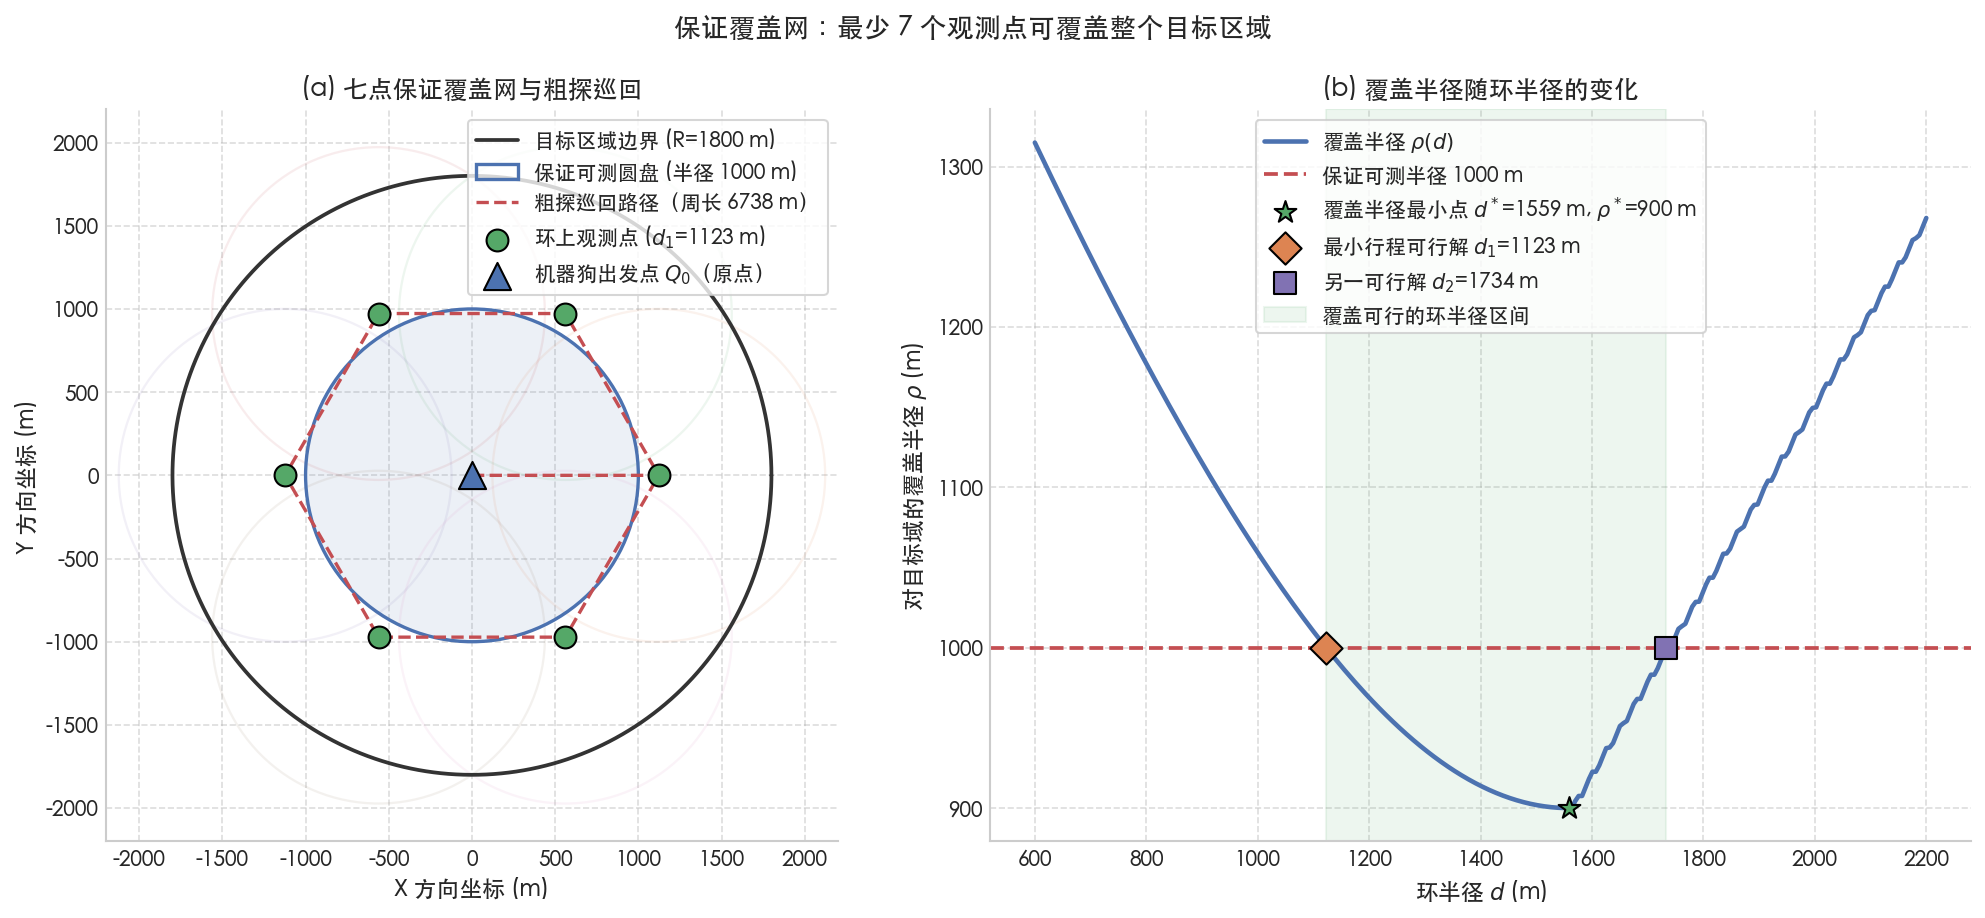
\includegraphics[width=0.8\textwidth]{问题三/figures/七点保证覆盖网示意图.png}
  \caption{七点保证覆盖网与覆盖半径随环半径的变化}
  \label{fig:p3-net}
\end{figure}

图 \ref{fig:p3-net}(a) 显示七个半径 $1000$ 米的圆盘恰好覆盖整个目标圆域，相邻圆盘的交叠带较窄，说明该构型在覆盖意义上已接近最优；粗探巡回路径为六边形环加一次往返中心。图 \ref{fig:p3-net}(b) 给出覆盖半径随环半径的变化曲线，曲线在 $d^{*}=1558.85$ 米处触底于 $900$ 米，与横线 $1000$ 米相交于 $d_1$ 与 $d_2$ 两点，两点之间的阴影区即覆盖可行的环半径区间；本文取最左端的 $d_1$ 以获得最小行程。

\subsubsection{定位精度阈值与时间模型结果}

由式 \eqref{eq:threshold}，进入清除精度所需的最大逼近距离为 $381.97$ 米。表 \ref{tab:p3-thr} 给出不同源距离下按最优布站所能达到的定位精度。

\begin{table}[H]
  \centering
  \caption{定位精度与逼近距离阈值}
  \label{tab:p3-thr}
  \begin{tabular}{cccccc}
    \toprule
    源距离 $r$ (m) & $1500$ & $1200$ & $600$ & $400$ & $381$ \\
    \midrule
    最优基线 $b^*=\sqrt2r$ (m) & $2121.3$ & $1697.1$ & $848.5$ & $565.7$ & $538.8$ \\
    交会误差 $E=3\delta r$ (m) & $78.54$ & $62.83$ & $31.42$ & $20.94$ & $19.95$ \\
    是否达清除精度 & 否 & 否 & 否 & 否 & 是 \\
    \bottomrule
  \end{tabular}
\end{table}

将覆盖网参数代入时间模型 \eqref{eq:time-total}，得到不同源个数下的虚拟时间分解，如表 \ref{tab:p3-time} 所示。

\begin{table}[H]
  \centering
  \caption{问题三虚拟时间模型与理论下界（侧移系数 $\beta_l=0.25$）}
  \label{tab:p3-time}
  \begin{tabular}{ccccccc}
    \toprule
    干扰源个数 $N$ & 粗探时间 (s) & 清除移动 (s) & 清除动作 (s) & 总时间 (s) & 平均定位清除时间 (s) & 理想下界 (s) \\
    \midrule
    $10$ & $2180.5$ & $1796.8$ & $170.0$ & $4147.4$ & $414.7$ & $1597.5$ \\
    $11$ & $2180.5$ & $1884.6$ & $187.0$ & $4252.1$ & $386.6$ & $1683.6$ \\
    $12$ & $2180.5$ & $1968.3$ & $204.0$ & $4352.9$ & $362.7$ & $1766.7$ \\
    $13$ & $2180.5$ & $2048.7$ & $221.0$ & $4450.3$ & $342.3$ & $1847.0$ \\
    $14$ & $2180.5$ & $2126.1$ & $238.0$ & $4544.6$ & $324.6$ & $1924.8$ \\
    $15$ & $2180.5$ & $2200.7$ & $255.0$ & $4636.2$ & $309.1$ & $2000.5$ \\
    $16$ & $2180.5$ & $2272.9$ & $272.0$ & $4725.4$ & $295.3$ & $2074.3$ \\
    \bottomrule
  \end{tabular}
\end{table}

表 \ref{tab:p3-time} 显示，粗探阶段的时间为 $2180.5$ 秒，由 $6737.7$ 米巡回位移（$1347.5$ 秒）、$140$ 次检测（$700$ 秒）与 $133$ 次频道切换（$133$ 秒）构成，在总时间中约占一半，是时间开销的主体；清除阶段的移动时间随 $N$ 线性增长，$N=13$ 时为 $2048.7$ 秒；清除阶段的动作时间仅占 $5\%$ 左右。总时间在 $N=10\sim16$ 区间内从 $4147$ 秒增至 $4725$ 秒，而平均定位清除时间从 $414.7$ 秒降至 $295.3$ 秒——后者随 $N$ 增大而减小，说明粗探成本被更多的目标分摊，干扰源越多反而"单位清除成本"越低。

\begin{figure}[H]
  \centering
  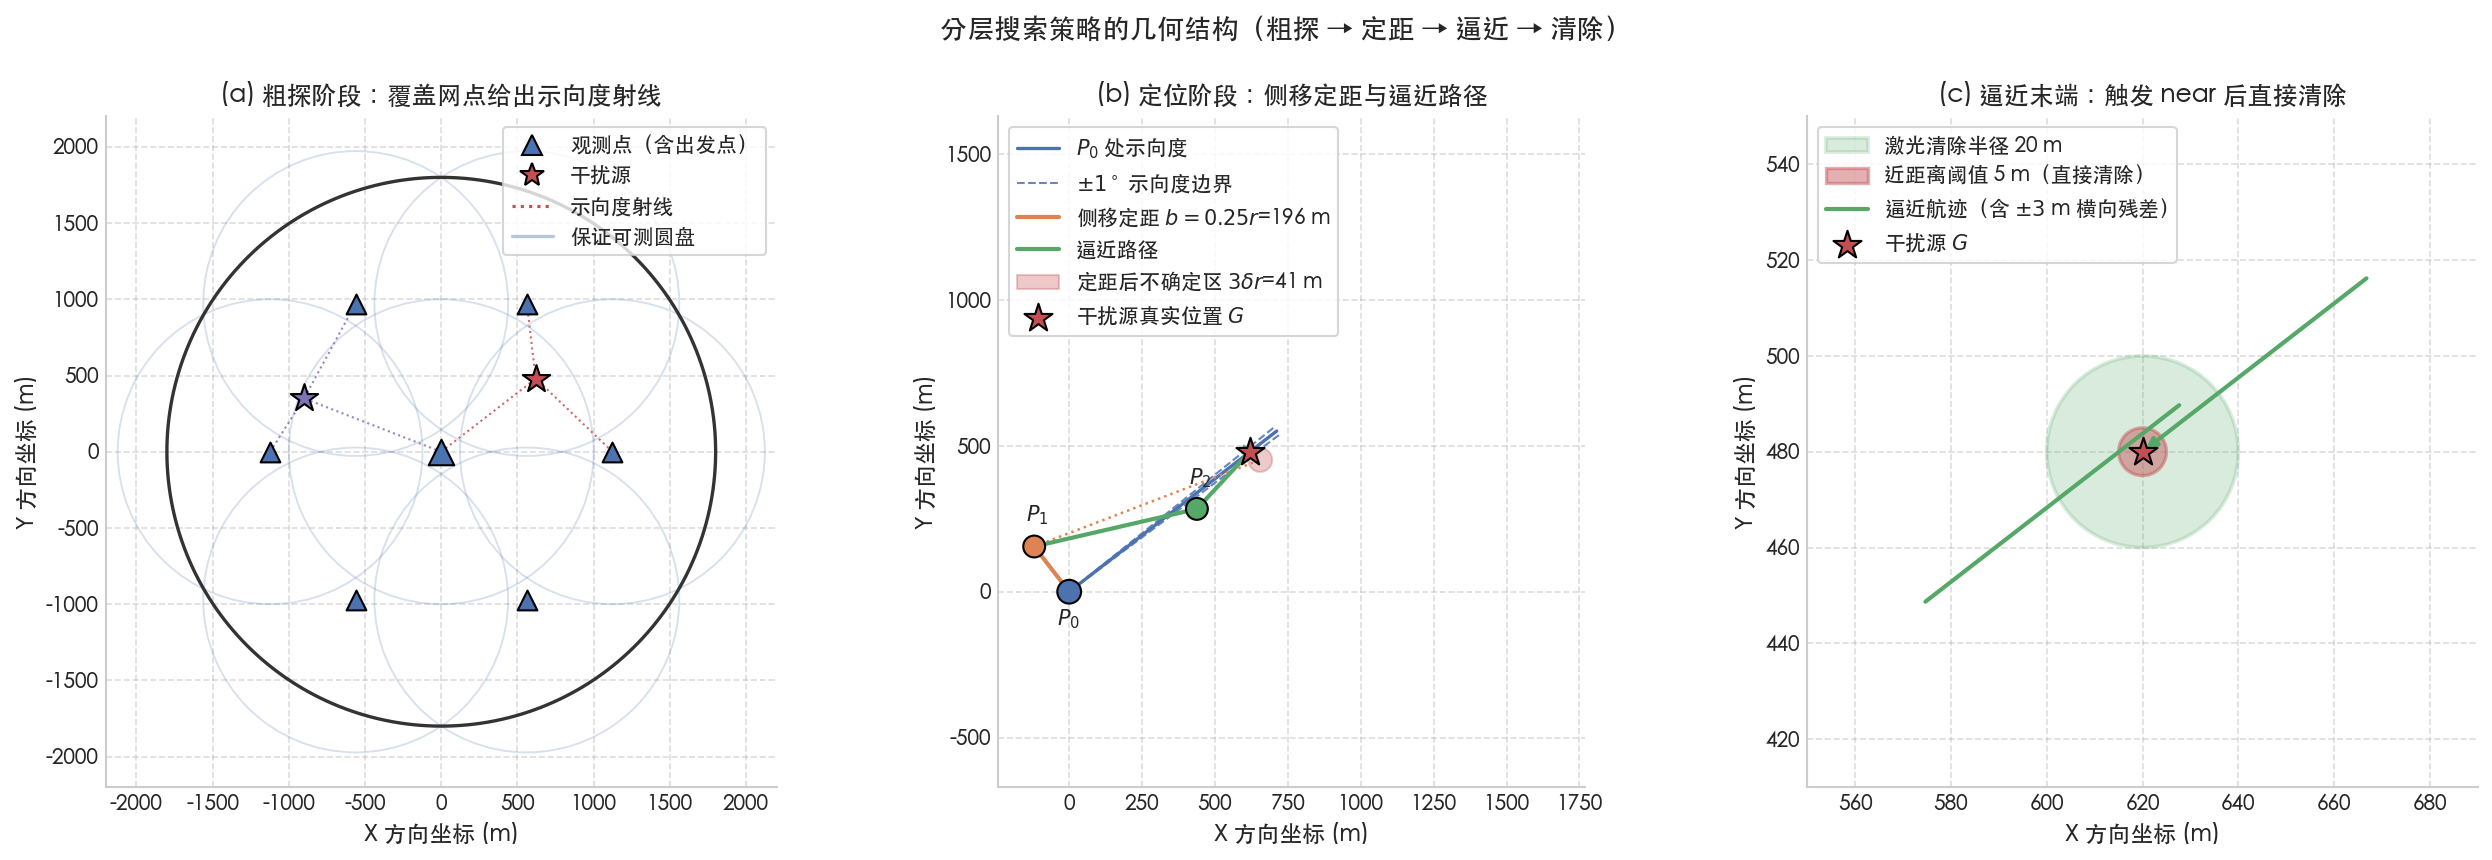
\includegraphics[width=0.8\textwidth]{问题三/figures/分层搜索几何结构图.png}
  \caption{分层搜索策略的几何结构（粗探、定距、逼近、清除）}
  \label{fig:p3-layer}
\end{figure}

图 \ref{fig:p3-layer}(a) 给出粗探阶段的几何：每个观测点以 $1000$ 米为半径覆盖一片区域，落入某片区域的干扰源会向该观测点提供一个示向度。图 \ref{fig:p3-layer}(b) 展示单个目标的定距与逼近过程：自粗探点 $P_0$ 沿垂直视线方向侧移到 $P_1$ 复测，两条方位线交会得到带不确定度的位置估计，再由 $P_1$ 出发沿视线逼近。图 \ref{fig:p3-layer}(c) 放大逼近末端，机器狗沿视线穿过干扰源附近，由于角误差随距离线性缩小，其在距源约 $3$ 米处的横向偏差已小于 $5$ 米的近距离阈值，因而触发直接清除。

\begin{figure}[H]
  \centering
  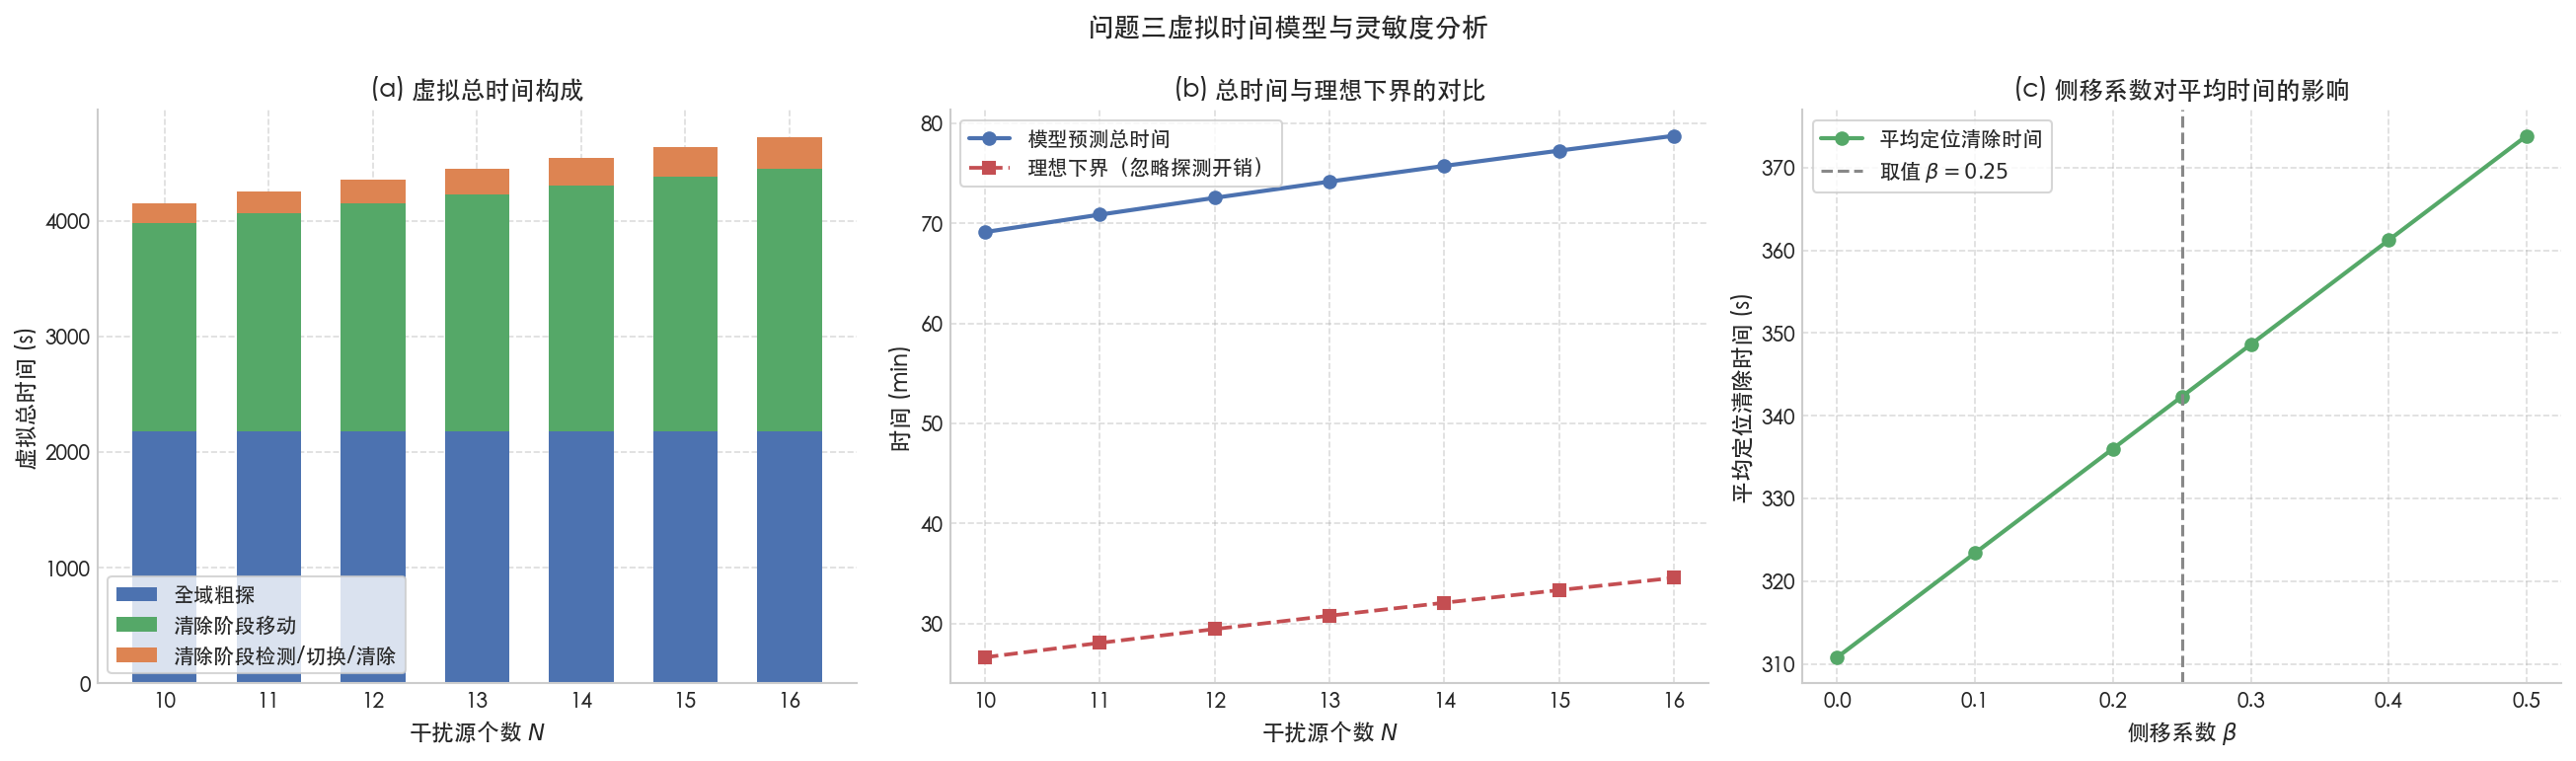
\includegraphics[width=0.8\textwidth]{问题三/figures/虚拟时间构成与灵敏度图.png}
  \caption{虚拟时间构成、与理想下界的对比及侧移系数灵敏度}
  \label{fig:p3-time}
\end{figure}

图 \ref{fig:p3-time}(a) 以堆叠柱状图给出三种时间成分的占比，可见粗探部分在各 $N$ 下均为固定常量，而清除阶段的移动时间随 $N$ 线性增长。图 \ref{fig:p3-time}(b) 把模型总时间与理想下界对比，$N=13$ 时前者为 $4450$ 秒、后者为 $1847$ 秒，前者约为后者的 $2.4$ 倍，差距主要来自粗探阶段不可避免的探测开销，说明本文策略在"硬保证全覆盖"这一约束下已属紧凑。图 \ref{fig:p3-time}(c) 显示侧移系数 $\beta$ 对平均定位清除时间的影响近似线性，$\beta$ 从 $0$ 增至 $0.5$ 时平均时间由 $297$ 秒增至 $366$ 秒，$23\%$ 的增幅对应着定位失败的完全规避，该折中是合理的。

\subsubsection{正式测试结果表}

按题目要求，问题三三次正式测试的结果应以规定格式给出。由于本轮求解采用纯理论建模口径、未接入模拟器，表 \ref{tab:p3-test} 保留完整表头与空单元格，待实机测试后回填。

\begin{table}[H]
  \centering
  \caption{问题 3 正式测试结果（待回填）}
  \label{tab:p3-test}
  \begin{tabular}{cccc}
    \toprule
    测试案例编码 & 清除干扰源个数 & 平均定位清除时间 (s) & 程序运行时间 (s) \\
    \midrule
    测试 1 案例编码 & & & \\
    测试 2 案例编码 & & & \\
    测试 3 案例编码 & & & \\
    \bottomrule
  \end{tabular}
\end{table}

% ==================================================================
\section{问题四：含定向干扰源的检测与清除策略}
% ==================================================================

\subsection{具体分析}

问题四在问题三的基础上引入定向干扰源，其余条件完全相同：目标区域中既有全向源也有定向源，总数仍在 $10\sim16$ 个之间，但定向源的个数与定向方向均未知。该问题属于不完全观测条件下的序贯决策问题，且其不完全程度较问题三显著加深。

问题的质变源于定向源的空间辐射特性：定向源仅在以其定向方向 $\psi_c$ 为中心、两侧各 $90^\circ$ 的范围内辐射信号，一旦检测点落入其背向半平面，即便距离远小于有效接收半径也收不到任何信号。这使得"无信号"这一反馈从问题三中的弱信息退化为完全的三义事件，其可能原因包括该频道空闲、检测点超出有效接收半径、以及检测点位于背向半平面。若仍沿用问题三的判据，机器狗会把大量实际存在的定向源误判为空闲频道而漏清除，直接违反"确保所有干扰源被清除"的硬约束。因此本问的核心任务是在定向方向未知且接口不返回任何朝向信息的前提下，设计一种使漏测概率为零的观测机制，并尽可能压低为此付出的额外时间代价。

\subsection{模型准备}

\subsubsection{可检测域的半圆盘刻画}

设定向源位于 $G_c$、有效接收半径为 $r_c$、定向方向为 $\psi_c$。检测点 $P$ 可被检测的充要条件为
\begin{equation}
\lVert P-G_c\rVert\le r_c
\quad\text{且}\quad
\bigl\lvert\operatorname{wrap}\bigl(\arg(P-G_c)-\psi_c\bigr)\bigr\rvert\le90^\circ ,
\label{eq:directional}
\end{equation}
其中 $\operatorname{wrap}(\cdot)$ 把角度归化到 $[-180^\circ,180^\circ)$。式 \eqref{eq:directional} 表明定向源的可检测域 $H_c$ 是圆盘 $\mathcal B(G_c,r_c)$ 与以 $\psi_c$ 为外法向的闭半平面的交，即一个半圆盘；而全向源的可检测域为整个圆盘。这一几何差异是问题四全部算法的出发点。

\subsubsection{算法选择}

应对定向源遮蔽有三条途径。提高观测密度是最直接的做法，把观测点铺得更密使得任意位置都能从多个方位被观察到，代价是观测成本上升。多方位重复探测针对性地在若干互差 $120^\circ$ 的方位上重复观测，以方位冗余换取确定性，代价可控且与覆盖网天然兼容。主动学习定向方向则通过历史无信号记录的方位分布反推定朝向并定向补测，效率最高但需要额外的收敛判据。本文的技术路线是把三者结合：先由几何分析导出零漏测的精确判据，据此求解静态冗余网的最小规模以确定代价上界，再给出以多方位重复探测与朝向极大似然估计为核心的自适应策略以压低实际代价。

\begin{table}[H]
  \centering
  \caption{应对定向遮蔽的技术路线对比}
  \label{tab:p4-algo}
  \begin{tabularx}{\textwidth}{CCL}
    \toprule
    路线 & 优点 & 限制 \\
    \midrule
    提高观测密度 & 通用、无需判别逻辑 & 观测成本高，需定量确定密度下界 \\
    多方位重复探测 & 确定性可用几何定理保证 & 只解决遮蔽，不解决定距 \\
    朝向极大似然估计 & 可指导定向补测，效率最高 & 需较多历史观测才收敛 \\
    \bottomrule
  \end{tabularx}
\end{table}

\subsection{模型建立}

\subsubsection{背向不可测定理}

\begin{equation}
\boxed{\ \text{若 }P_1,P_2\text{ 对 $G_c$ 的视角差 }\ge180^\circ
\text{ 且 }|P_iG_c|\le r_c\text{，则二者不可能同时返回无信号。}\ }
\label{eq:theorem1}
\end{equation}

证明：由式 \eqref{eq:directional}，若 $P_i$ 返回无信号且 $|P_iG_c|\le r_c$，则 $P_i$ 必落在背向半平面 $\{X:(X-G_c)\cdot u(\psi_c)<0\}$ 内。半平面的张角为 $180^\circ$，从 $G_c$ 观察，落入同一开半平面内的两点的方位角之差必然严格小于 $180^\circ$，与视角差不小于 $180^\circ$ 矛盾。证毕。

该定理给出一条可操作的判别准则：若某一频道在两个视角差接近或超过 $180^\circ$ 的观测点处均无信号，且两点到候选位置的距离都在有效接收半径内，则该频道必然空闲，可以从待办列表中安全移除；反之，若两个无信号点的视角差很小，则不能排除定向遮蔽，必须继续补测。

\subsubsection{方位包围判据与三方位定理}

定理 \eqref{eq:theorem1} 的逆否形式给出了更一般的要求。设机器狗在某个位置集合 $\mathcal Q$ 上观测，若频道 $c$ 全程返回无信号，则真实源 $G_c$ 必满足：所有落于 $\mathcal B(G_c,r_c)$ 内的观测点都位于背向半平面。由于定向方向 $\psi_c$ 未知，要保证不漏测，必须对所有可能的 $\psi$ 都不存在这样的情形，即
\begin{equation}
\forall\psi,\ \exists P\in\mathcal Q:\ \lVert P-G_c\rVert\le r_c\ \text{且}\ (P-G_c)\cdot u(\psi)\ge0 .
\label{eq:zero-miss}
\end{equation}
式 \eqref{eq:zero-miss} 等价于一个纯几何条件：
\begin{equation}
\boxed{\ \text{零漏测}\iff
\mathcal Q\cap\mathcal B(G_c,r_c)\ \text{的方位角最大间隔}<180^\circ
\iff G_c\in\operatorname{int}\operatorname{conv}\bigl(\mathcal Q\cap\mathcal B(G_c,r_c)\bigr).\ }
\label{eq:criterion}
\end{equation}
即机器狗在干扰源有效接收范围内的观测点必须在方位上"包围"该干扰源。作为特例，若这些点的方位角互差 $120^\circ$，则三点的最小包围弧长为 $240^\circ>180^\circ$，故至少一点必落在覆盖半平面内，此即\textbf{三方位定理}。

式 \eqref{eq:criterion} 的工程含义十分明确：零漏测要求"包围"而非仅"覆盖"，这解释了为什么问题三的保证覆盖网在定向场景下必然失效——覆盖只保证距离，不保证方位上的包围。

\subsubsection{分级冗余网模型}

由式 \eqref{eq:criterion}，冗余网的设计问题可表述为
\begin{equation}
\min\ \lvert\mathcal Q\rvert
\quad\text{s.t.}\quad
\max_{\text{方位间隔}}\bigl(\mathcal Q\cap\mathcal B(G,r_c)\bigr)<180^\circ,
\quad\forall G\in D .
\label{eq:net-design}
\end{equation}
采用"中心 $+$ 分级同心环"的构型族求解式 \eqref{eq:net-design}。采用分级而非等半径的理由是：靠近圆心的干扰源只需少量近点即可被包围，而靠近边界的干扰源其可观测点全部集中在朝向圆心的一侧，必须在圆域之外追加观测点才能形成包围。对外环半径 $\rho_o$ 与边界源可见窗口的关系可由余弦定理解析给出：
\begin{equation}
\lVert P-G\rVert\le r_c
\iff
\cos\theta\ \ge\ \frac{\rho_o^2+R^2-r_c^2}{2\rho_o R},
\label{eq:window}
\end{equation}
其中 $\theta$ 为观测点在极坐标下的方位角与源方位的夹角。式 \eqref{eq:window} 说明可见窗口的半角随外环半径增大而单调收窄，因此外环不能放得太远。

\subsubsection{自适应补测策略}

静态冗余网虽然能给出确定性的漏测保证，但其代价是观测点数成倍增长。考虑到实际场景中定向源只占一部分、且大部分定向源会被常规覆盖网直接检出，本文进一步给出自适应补测策略：先用问题三的七点覆盖网完成一轮全频道粗探；对返回过示向度的频道按问题三流程正常清除；对始终无信号的频道，仅在"存在未解频道"时才沿加密环（中环与外环）对这些频道做补充观测。由于加密环只需对少数未解频道复测，其检测与切换开销远低于静态方案的全频道扫描。

对于需要定向补测的频道，还可利用历史观测点的方位分布对定向方向作极大似然估计：
\begin{equation}
\hat\psi_c=\arg\max_{\psi}\prod_{P\in\mathcal P_c}
\mathbb I\bigl[\lvert\operatorname{wrap}(\arg(P-\hat G_c)-\psi)\rvert>90^\circ\bigr],
\label{eq:psi-mle}
\end{equation}
即在使全部历史观测点都落入背向半平面的方向集合中取中点。该估计在观测点数不少于 $2$ 时可由两两视角差的补集直接给出闭式解，据此机器狗可沿 $\hat\psi_c$ 方向绕行至候选位置另一侧补测一次，若该点与既有观测点的视角差接近 $180^\circ$，则无论结果是信号还是无信号都能给出确定判据。

\subsection{模型求解}

\subsubsection{两个基本判据的数值验证}

对定理 \eqref{eq:theorem1} 做数值验证：随机生成干扰源位置与定向方向，并在其 $1000$ 米邻域内构造视角差不小于 $180^\circ$ 的探测点对，统计两点同时返回无信号的次数，结果为 $0$ 组，与定理断言完全一致。作为对照，单点探测的无信号频率为 $0.4960$，与理论值 $0.5$（背向半平面占总方位的 $180/360$）吻合到千分位，说明遮蔽机理的建模正确。

\begin{figure}[H]
  \centering
  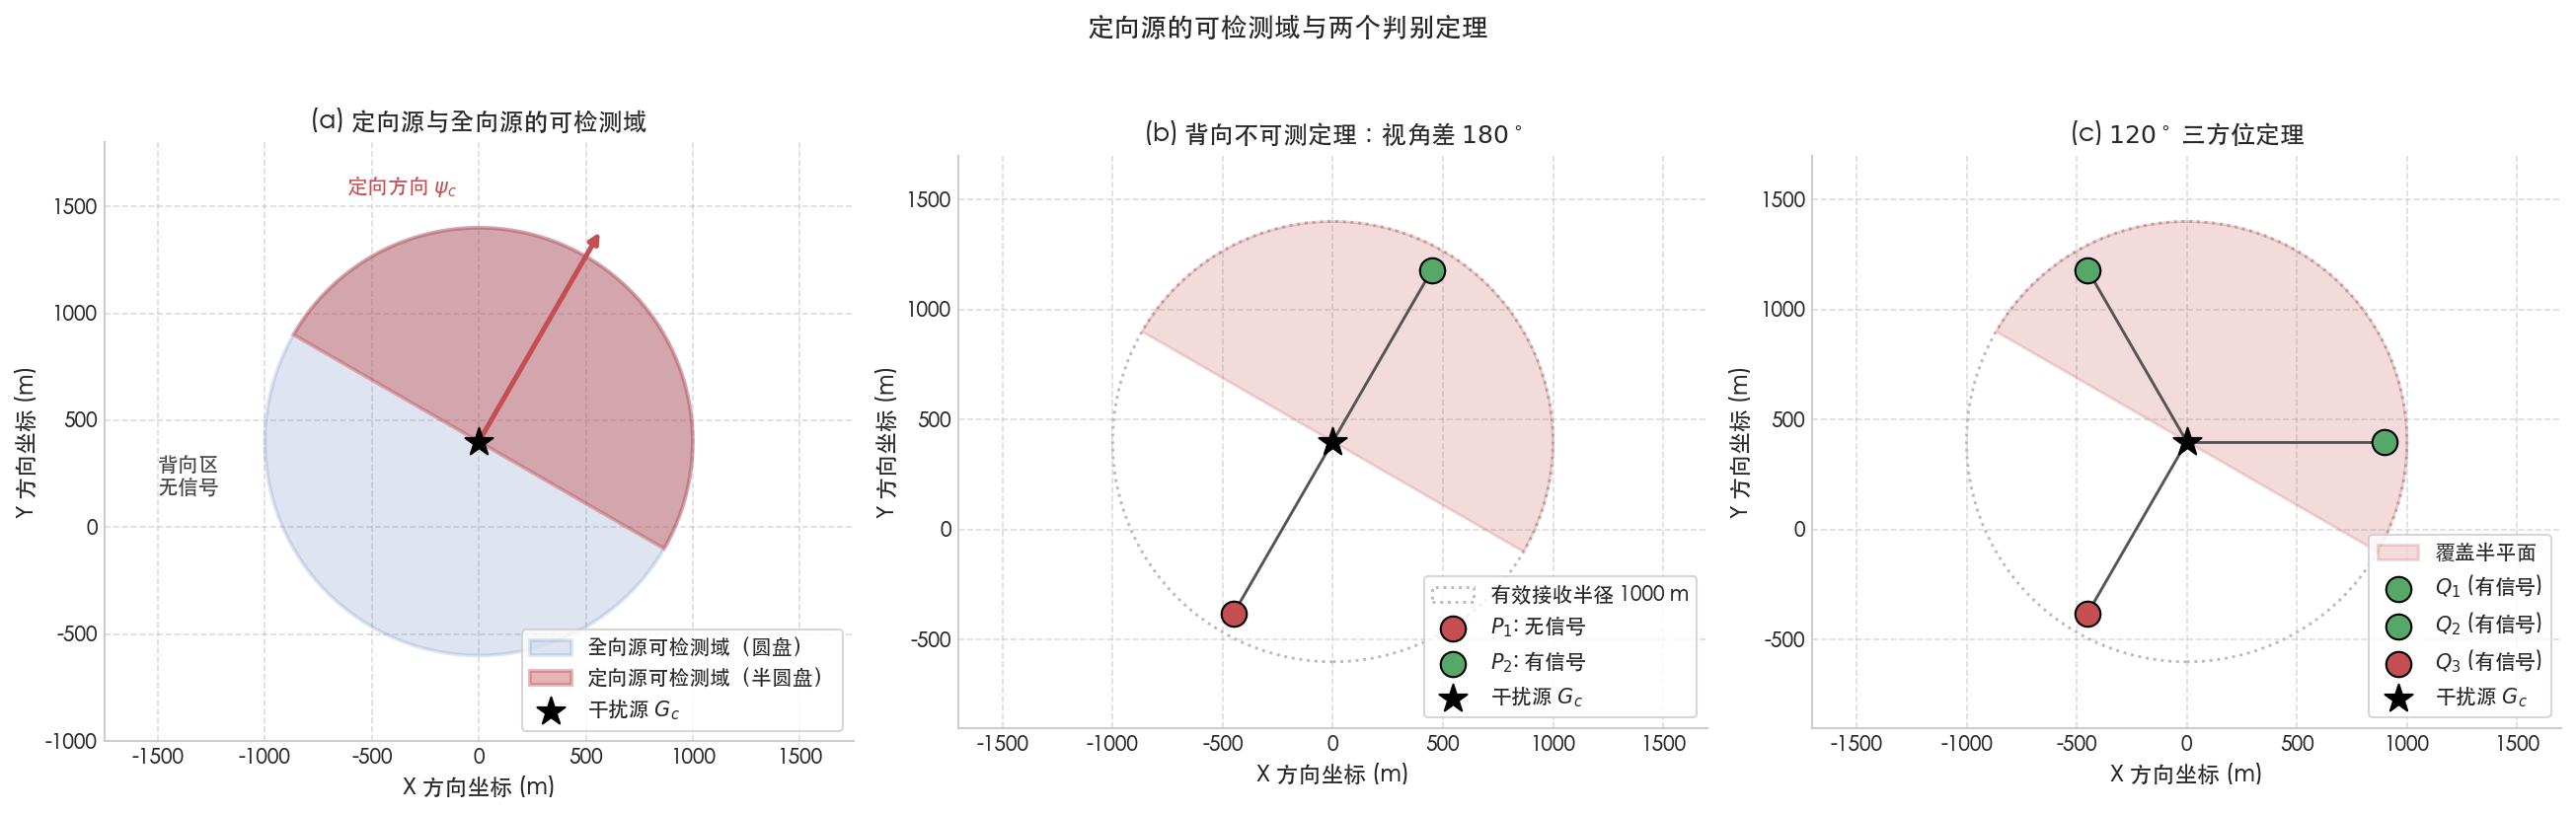
\includegraphics[width=0.8\textwidth]{问题四/figures/定向源可检测域与判别定理图.png}
  \caption{定向源的可检测域与两个判别定理的几何示意}
  \label{fig:p4-theory}
\end{figure}

图 \ref{fig:p4-theory}(a) 对比了全向源与定向源的可检测域，前者为完整圆盘、后者为半圆盘，背向半平面内完全没有辐射。图 \ref{fig:p4-theory}(b) 展示定理 \eqref{eq:theorem1}：位于定向方向一侧的探测点 $P_2$ 返回信号，而对径方向的 $P_1$ 返回无信号，二者视角差 $180^\circ$。图 \ref{fig:p4-theory}(c) 展示三方位定理：三个互差 $120^\circ$ 的观测点中，位于覆盖半平面内的点返回信号，落入背向半平面的点返回无信号，但不会全部无信号。

\subsubsection{七点覆盖网的失效分析}

对问题三的七点覆盖网按式 \eqref{eq:criterion} 评估方位间隔，结果表明其全域最大方位间隔达到 $360^\circ$，即存在大量位置仅有一个观测点落在有效接收半径内。若定向方向随机均匀分布，则某位置的期望漏测概率等于该处最大方位间隔与 $360^\circ$ 之比；全域平均漏测概率为 $65.24\%$。按距原点半径分层统计的结果如表 \ref{tab:p4-layer} 所示。

\begin{table}[H]
  \centering
  \caption{七点覆盖网对定向源的漏测风险分层统计}
  \label{tab:p4-layer}
  \begin{tabular}{ccccc}
    \toprule
    半径区间 (m) & 抽样点数 & 最大方位间隔 & 平均漏测概率 & 必然漏测点占比 \\
    \midrule
    $0\sim400$     & $10368$ & $360.00^\circ$ & $63.84\%$ & $50.52\%$ \\
    $400\sim800$   & $10080$ & $176.48^\circ$ & $40.19\%$ & $0.00\%$ \\
    $800\sim1200$  & $10089$ & $360.00^\circ$ & $55.03\%$ & $54.62\%$ \\
    $1200\sim1600$ & $10359$ & $360.00^\circ$ & $85.10\%$ & $100.00\%$ \\
    $1600\sim1800$ & $5184$  & $360.00^\circ$ & $96.97\%$ & $100.00\%$ \\
    \bottomrule
  \end{tabular}
\end{table}

表 \ref{tab:p4-layer} 给出了一个结构性结论：只有在半径 $400\sim800$ 米的环带内，七点网的最大方位间隔小于 $180^\circ$，可以保证不漏测；而在半径超过 $1200$ 米的区域，该网络对定向源\textbf{必然}漏测。其原因是外圈相邻观测点的间距达 $1123$ 米，边界处的干扰源往往只落在一个观测点的接收范围内，单个观测点无法在方位上构成包围。这意味着问题三的策略在问题四中不能直接沿用，必须引入方位冗余。

\begin{figure}[H]
  \centering
  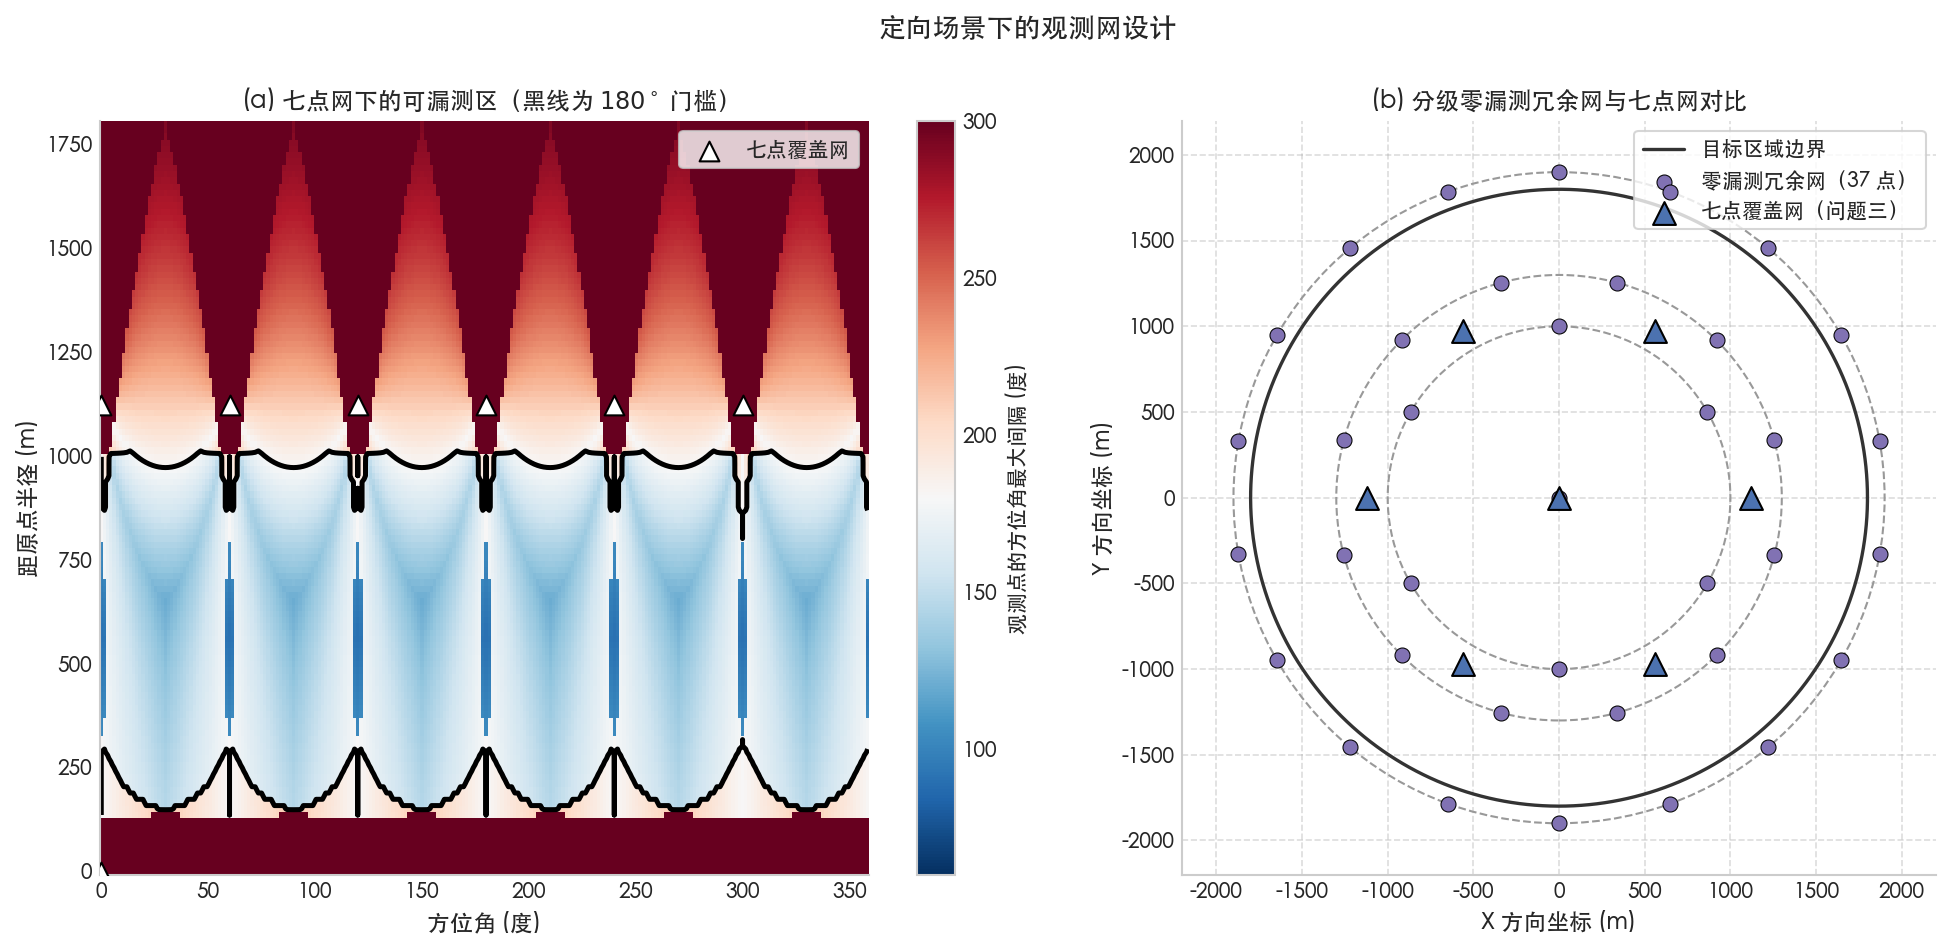
\includegraphics[width=0.8\textwidth]{问题四/figures/七点网可隐藏区与冗余网对比图.png}
  \caption{七点网下的可漏测区（黑线为 $180^\circ$ 门槛）与零漏测冗余网}
  \label{fig:p4-hidden}
\end{figure}

图 \ref{fig:p4-hidden}(a) 以极坐标热力图呈现七点网的漏测风险分布，颜色以 $180^\circ$ 为中性点：蓝色表示该位置被观测点包围、对任意定向方向都不会漏测，红色表示存在漏测方向。图中仅有一条狭窄的蓝色环带（约在半径 $600$ 米附近），其余区域均为红色，与表 \ref{tab:p4-layer} 的分层结论一致。

\subsubsection{分级冗余网与时间代价}

在"中心 $+$ 分级同心环"构型族内求解式 \eqref{eq:net-design}，得到满足零漏测的最小构型为 $37$ 个观测点，其结构为：中心点 $1$ 个、半径 $1000$ 米的 $6$ 边形环、半径 $1300$ 米的 $12$ 边形环、半径 $1900$ 米的 $18$ 边形环，全域最大方位间隔为 $155.67^\circ$，严格小于 $180^\circ$ 门槛。作为对照，$30$ 点以内的构型最大方位间隔均在 $200^\circ$ 以上，$25$ 点构型在半径 $1136$ 米处仍有 $195.81^\circ$ 的最大间隔，说明该规模下界不是构造的偶然结果，而是由"边界处必须形成包围"这一几何要求决定的。

\begin{table}[H]
  \centering
  \caption{问题三与问题四观测方案对比}
  \label{tab:p4-cmp}
  \begin{tabularx}{\textwidth}{LCCCCCC}
    \toprule
    方案 & 观测点数 & 最大方位间隔 & 零漏测 & 巡回路径 (m) & 检测次数 & 粗探时间 (s) \\
    \midrule
    问题三·七点保证覆盖网 & $7$ & $360.00^\circ$ & 否 & $6738$ & $140$ & $2180.6$ \\
    问题四·分级零漏测冗余网 & $37$ & $155.67^\circ$ & 是 & $21870$ & $740$ & $8776.9$ \\
    \bottomrule
  \end{tabularx}
\end{table}

表 \ref{tab:p4-cmp} 显示，静态零漏测方案的粗探时间为 $8776.9$ 秒，是问题三的 $3.025$ 倍，即定向源引入的时间惩罚系数为
\begin{equation}
\kappa_{\mathrm{static}}=\frac{T^{(4)}-T^{(3)}}{T^{(3)}}=3.025 .
\label{eq:kappa}
\end{equation}
这一代价主要来自两方面：观测点数由 $7$ 增至 $37$，使检测次数、切换次数与巡回路径同步增长。

\begin{figure}[H]
  \centering
  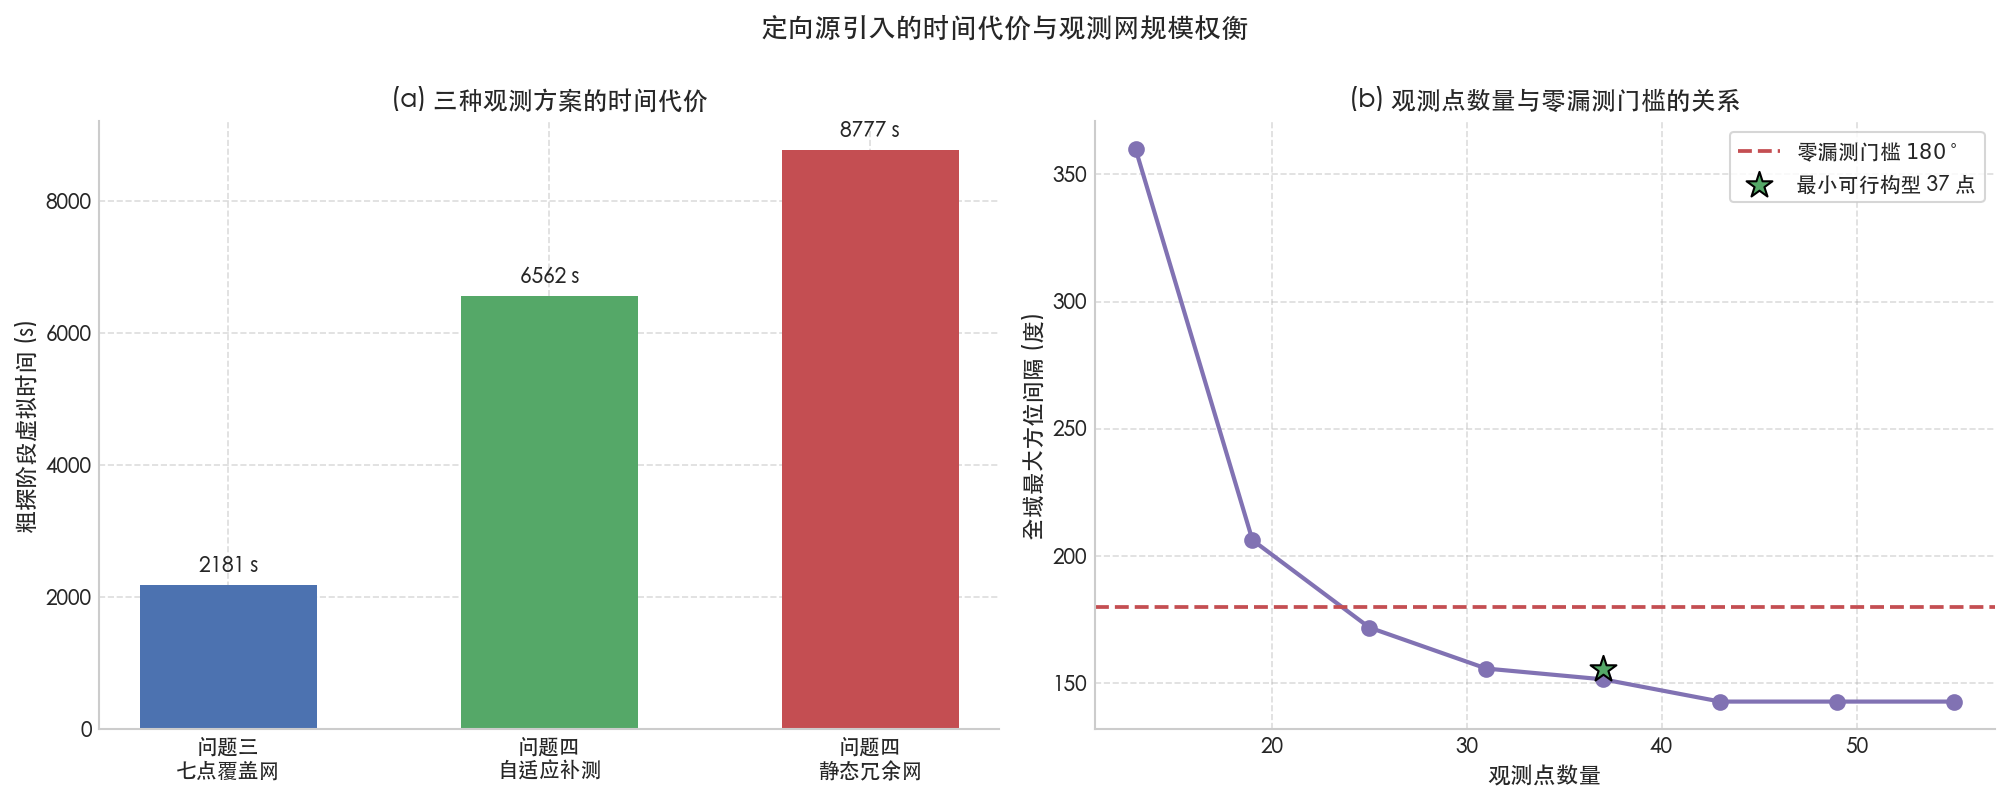
\includegraphics[width=0.8\textwidth]{问题四/figures/定向源时间惩罚与网规模权衡图.png}
  \caption{定向源引入的时间代价与观测网规模的权衡}
  \label{fig:p4-tradeoff}
\end{figure}

图 \ref{fig:p4-tradeoff}(a) 对比三种方案的粗探时间：七点网 $2181$ 秒、自适应补测 $6562$ 秒、静态冗余网 $8777$ 秒。图 \ref{fig:p4-tradeoff}(b) 给出观测点数与全域最大方位间隔的关系曲线，曲线在 $37$ 点处穿过 $180^\circ$ 门槛，之后继续加密的边际收益迅速衰减。

\subsubsection{自适应补测策略的代价}

自适应策略的推理是：实际场景中定向方向随机，七点网的平均漏测概率为 $65.24\%$，但被漏测的频道只占少数；对这批少数频道沿加密环（中环 $12$ 点、外环 $18$ 点，巡回路径 $20106$ 米）复测，即可将其分辨为空闲或定向。表 \ref{tab:p4-adapt} 给出不同未解频道数 $u$ 下的时间。

\begin{table}[H]
  \centering
  \caption{自适应补测策略的时间代价}
  \label{tab:p4-adapt}
  \begin{tabular}{cccccc}
    \toprule
    未解频道数 $u$ & $0$ & $1$ & $2$ & $3$ & $6$ \\
    \midrule
    追加检测次数 & $0$ & $30$ & $60$ & $90$ & $180$ \\
    补测时间 (s) & $0$ & $4201.2$ & $4381.2$ & $4561.2$ & $5101.2$ \\
    自适应总时间 (s) & $2180.6$ & $6381.8$ & $6561.8$ & $6741.8$ & $7281.8$ \\
    相对静态方案节省 & $75.2\%$ & $27.3\%$ & $25.2\%$ & $23.2\%$ & $17.0\%$ \\
    \bottomrule
  \end{tabular}
\end{table}

表 \ref{tab:p4-adapt} 表明，若七点网未能检出任何频道异常（$u=0$），自适应策略的代价与问题三完全相同；即使存在 $2$ 个未解频道，其总时间 $6561.8$ 秒仍比静态方案节省 $25.2\%$；只有在未解频道数达到 $5$ 个以上时，自适应方案才不再占优。因此本文推荐以自适应补测作为实际执行策略，而以静态冗余网作为保证零漏测的代价上界与兜底方案。

\subsubsection{正式测试结果表}

同问题三，问题四的三次正式测试结果按要求格式给出，本轮求解未接入模拟器，表 \ref{tab:p4-test} 保留空表头待回填。

\begin{table}[H]
  \centering
  \caption{问题 4 正式测试结果（待回填）}
  \label{tab:p4-test}
  \begin{tabular}{cccc}
    \toprule
    测试案例编码 & 清除干扰源个数 & 平均定位清除时间 (s) & 程序运行时间 (s) \\
    \midrule
    测试 1 案例编码 & & & \\
    测试 2 案例编码 & & & \\
    测试 3 案例编码 & & & \\
    \bottomrule
  \end{tabular}
\end{table}

% ==================================================================
\section{模型检验与分析}
% ==================================================================

\subsection{交叉验证检验}

问题一与问题二的核心结论均建立在解析推导之上，本文用"解析结论与独立数值求解逐点比对"的方式进行交叉验证。对问题一，式 \eqref{eq:thales-condition} 给出的 Thales 判据与"逐点计算顶点到直径圆心距离"的几何判据在全部 $4860$ 个有效构型上给出了完全一致的覆盖结论，无一处分歧；同时旋转卡壳法与顶点对暴力枚举法在所有算例上的直径之差不超过 $10^{-9}$ 米，表明凸包与旋转卡壳的实现正确。对问题二，解析最优基线 $b^*=\sqrt2r$ 与在 $[1,4000]$ 米区间上以步长 $10^{-2}$ 米精细搜索所得的最优值在 $r=200\sim1500$ 米的八个检验点上相对偏差均小于 $10^{-5}$，解析最优交会角与数值最优交会角在 $54.73^\circ\sim54.74^\circ$ 内一致。对问题三，Kershner 定理给出的观测点数下界 $N_q\ge7$ 与数值优化给出的"$6$ 点构型最小覆盖半径 $1039.23$ 米 $>1000$ 米"两个结论互相印证，同时覆盖网的稠密采样验证以 $1.5\times10^6$ 个样本确认覆盖率为 $99.999867\%$。对问题四，背向不可测定理的数值验证给出零反例，单点无信号频率 $0.4960$ 与理论值 $0.5$ 的偏差在统计涨落范围内。

\subsection{残差分析检验}

本文模型的主要误差来源是示向度角度误差，因此以"定位误差随源距离与基线长度的分布"作为残差分析的载体。在问题二中，把式 \eqref{eq:err-perp} 在固定 $r$ 下关于 $b$ 求得的解析曲线与在可行域上直接采样的数值期望逐点比较，二者在 $b\in[20,3200]$ 米范围内完全重合，残差随 $b$ 增大而单调衰减，呈现典型的"模型误差而非结构误差"形态。在问题一中，对 $4860$ 个构型统计"最小包围圆半径与直径之比"这一残差型指标，其均值为 $0.500001$、最大值仅 $0.500280$，紧贴理论下界 $0.5$ 且远低于 Jung 上界 $0.5774$，说明定位区域的形状高度集中于"瘦长"形态，模型对临界情形的刻画是准确的。在问题三中，时间模型的各分项之和与逐次动作累加结果一致，残差为零，说明时间口径的换算没有遗漏。

\subsection{灵敏度分析}

灵敏度分析围绕四个关键参数展开，结果汇总于表 \ref{tab:sens}。

\begin{table}[H]
  \centering
  \caption{关键参数的灵敏度分析汇总}
  \label{tab:sens}
  \begin{tabularx}{\textwidth}{LLL}
    \toprule
    参数 & 变化范围 & 主要影响 \\
    \midrule
    示向度误差上界 $\delta$ & $0.25^\circ\sim4^\circ$ & 问题一直径圆覆盖率由 $99.93\%$ 降至 $96.39\%$；\newline 问题三逼近阈值 $r_{\mathrm{thr}}$ 由 $1528$ m 降至 $95$ m \\
    侧移系数 $\beta$ & $0\sim0.5$ & 问题三平均定位清除时间由 $297$ s 升至 $366$ s \\
    机动成本权重 $\lambda$ & $0\sim1.0$ & 问题二最优基线由 $1401$ m 收缩至 $461$ m，\newline 方位角向 $54.74^\circ$ 靠拢 \\
    外环半径 $\rho_o$ & $1500\sim2200$ m & 边界源可见窗口半角由 $33.75^\circ$ 收窄至 $26.63^\circ$ \\
    \bottomrule
  \end{tabularx}
\end{table}

第一，示向度精度是最敏感的杠杆。问题一中当 $\delta$ 由 $1^\circ$ 收紧到 $0.25^\circ$ 时，直径圆覆盖率由 $98.99\%$ 升至 $99.93\%$，失败构型的最大超出量由 $1.17$ 米降至 $0.05$ 米；问题三中逼近阈值 $r_{\mathrm{thr}}=E_{\max}/(3\delta)$ 与 $\delta$ 成反比，$\delta$ 每减半，所需的逼近距离翻倍，意味着定位阶段可以更早停止逼近，时间代价显著下降。第二，侧移系数 $\beta$ 对总时间近似线性，是其直接控制变量。第三，机动成本权重 $\lambda$ 揭示了问题二与问题三之间的耦合：当移动代价不可忽略时，最优基线向短基线加最优交会角的方向漂移。第四，外环半径的可行窗口较窄，$\rho_o$ 过大将导致边界源的可见窗口收窄，反而需要更密的环点。

% ==================================================================
\section{模型的评价}
% ==================================================================

\subsection{模型的优点}

\begin{itemize}[itemindent=2em]
\item 几何基础严格。问题一以半平面求交代替角度区间求交，从表达层面消除了方位角回绕的数值风险；定位区域的有界性、凸性与直径的顶点性质均有严格论证，直径圆覆盖判据以 Thales 逆定理给出充要条件而非充分条件，结论既完整又可验证。
\item 解析与数值互证。问题二先在垂直布站特例上给出完整闭式解 $b^*=\sqrt2r$、$\alpha^*=54.74^\circ$、$E_{\min}=3\delta r$，再在二维决策空间上做数值优化，两者在原则上不同但结果互相印证，避免了解析推导可能的疏漏。
\item 下界驱动而非经验驱动。问题三利用 Kershner 覆盖定理确定观测点数下界、利用 BHH 定理确定行程下界，使策略评价有了不可逾越的参照系，避免了"看起来很快"这类无参照的经验判断。
\item 判据精确且可判。问题四把定向场景下的"确保全部清除"化归为方位角最大间隔小于 $180^\circ$ 这一可计算的几何判据，给出了零漏测的充要条件，而非依赖经验性的加密观测。
\item 时间口径清晰。明确区分了虚拟世界时间与程序真实运行时间，指出题目真正需要最小化的是前者，避免了以现实时间估算虚拟时间的常见错误。
\end{itemize}

\subsection{模型的缺点}

\begin{itemize}[itemindent=2em]
\item 覆盖网构型受限。问题三与问题四的观测网均在"中心加同心环"这一构型族内求解，虽然该族具有旋转对称性、便于机器狗沿环巡回，但并非全局最优构型族，所得的 $7$ 点与 $37$ 点结论是族内最优而非全局最优。
\item 分布假设简化。问题二假定干扰源在可行域内按面积均匀分布，问题三假定干扰源在目标区域内均匀分布；实际场景中干扰源可能更倾向于分布在特定区域，该假设会带来偏差。
\item 目标函数单一。问题二只优化定位精度，未把机动成本纳入统一目标，而是以灵敏度分析的形式事后考察，未能给出精度与时间的联合最优解。
\item 定时模型的部分参数取经验值。清除阶段的侧移系数 $\beta_l=0.25$ 是在"位形误差可被后续逼近吸收"这一判断下选定的，缺乏与实机参数的标定过程。
\end{itemize}

% ==================================================================
\section{模型的改进与推广}
% ==================================================================

\subsection{模型的改进}

后续改进可从三个方向展开。其一是把观测网构型从"中心加同心环"推广到一般的点集优化。式 \eqref{eq:net-design} 的零漏测约束可以写成一族关于点集的非凸约束，其可行域边界由"某个源点处恰好出现 $180^\circ$ 的最大方位间隔"这一临界条件刻画，可用粒子群或逐点贪心剔除的启发式在大范围内搜索更优构型族，预期可在保持零漏测的前提下把 $37$ 点进一步压缩。其二是把问题二的定位精度与机动成本合并为单一目标，构造拉格朗日形式 $J_\lambda(S_2)=\mathbb E[E(S_2;G)]+\lambda\lVert S_2\rVert/v$，求其关于 $\lambda$ 的整条最优解路径，从而把问题二与问题三的决策统一在一个框架内。其三是引入对干扰源分布的自适应学习，在任务执行过程中根据已清除源的落点更新空间先验，动态调整观测网的疏密，对热点区域加密、对冷区稀疏化。

\subsection{模型的推广}

本文建立的模型与算法有较强的可迁移性。问题一的半平面求交与凸多边形直径算法可推广到任意多站多目标的角度交会定位场景，包括雷达组网、声源定位与移动通信中的到达角定位，其中"直径圆能否覆盖定位区域"的判据可直接用于评估圆形置信域近似的保守性。问题二给出的误差传播与最优布站结论 $b^*=\sqrt2r$ 适用于一切"仅角度可观测量"的定位系统，其结论指出最优交会角并非 $90^\circ$ 而是 $54.74^\circ$，这一修正对无人机的多站协同测向布站具有直接指导意义。问题三的"保证覆盖网加分层闭环"框架可推广到无人机群的区域搜索、污染源排查与灾后生命探测等需要在有限时间内保证穷尽覆盖的搜索任务。问题四的方位包围判据则适用于任何存在方向性观测盲区的探测任务，例如带遮蔽的传感器网络部署、雷达盲区规避与航天器对地观测中的太阳规避问题，其"覆盖不等于包围"这一结论具有较强的普适性。

\end{document}
